\documentclass[Master, ngerman, UKenglish, bibstyle=alphabetic]{scrbook}
%------------------------------------------------------------------------------
% This file contains a skeleton thesis for
% a Physics or Astronomy Institute in the University of Bonn.

% Specify the thesis type as an option: PhD, Master, Diplom, Bachelor.
% Specify the thesis stage as an option: Draft (default), Submit, Final, PILibrary.

% Specify the language(s) in the class and then use babel.
% If you need more than one language, give the default language last,
% e.g. ngerman, UKenglish for a thesis in British (UK) English where you want
% to be able to set the language to German for some part of it.

%------------------------------------------------------------------------------
% Pass TeX Live version to the package.
% Use command pdflatex --version to find out which version you are running.
% twoside=true is suitable for printing, while twoside=false is probably better for PDF version.
\usepackage[twoside=true, texlive=2017]{ubonn-thesis}

%------------------------------------------------------------------------------
% Adjustments to standard biblatex style.
% Change option to backref=false when your thesis is ready to turn off back-referencing.
% Pass the option showurl=false to shorten your bibliography by not including url fields.
\usepackage[backref=true]{ubonn-biblatex}

%------------------------------------------------------------------------------
% Glossary package
% \usepackage[acronym,toc,nosuper]{glossaries}
% TikZ packages and libraries
% \usepackage{tikz}
% \usepackage{tikz-3dplot}
% \usepackage{pgfplots}
% \usetikzlibrary{positioning,shapes,arrows}
% \usetikzlibrary{decorations.pathmorphing}
% \usetikzlibrary{decorations.markings}
\usepackage{thesis_defs}

%------------------------------------------------------------------------------
% Instead of colouring  links, cites, table of contents etc.
% put them in a coloured box for the screen version.
% This is probably a good idea when you print your thesis.
\hypersetup{colorlinks=false,
   linkbordercolor=blue,citebordercolor=magenta,urlbordercolor=darkgreen
 }

%------------------------------------------------------------------------------
% When writing your thesis it is often helpful to have the date and
% time in the output file. Comment this out for the final version.
\ifoot[\today{} \thistime]{\today{} \thistime}

% In order to check if your labels are referenced try the refcheck package
% \usepackage{refcheck}

%------------------------------------------------------------------------------
% biblatex is included by ubonn-thesis. Look there for the settings used.
% See the options for settings that can be changed easily.
% For further changes copy the \RequirePackage[...]{biblatex} here
% and include ubonn-thesis with the option biblatex=false.

% Specify the bibliography files here and not at the end!
% Use standard_refs-bibtex if you use bibtex or bibtex8
% and standard_refs-biber  if you use biber
%\addbibresource{bib/thesis_refs.bib}
\addbibresource{bib/standard_refs-biber.bib}

%------------------------------------------------------------------------------
% The following definitions are used to produce the title pages
% needed at various stages
\newcommand{\thesistitle}{Determination of the beam asymmetry $\Sigma$ in $\eta'$ photoproduction}
\newcommand*{\thesisauthor}{\textsc{Jakob Michael Krause}}
\newcommand*{\thesistown}{Vechta}
\renewcommand*{\InstituteName}{\HISKP}
\renewcommand*{\inInstitute}{\inHISKP}
\renewcommand*{\InstituteAddress}{\HISKPaddress}
% Adjust \thesisreferee...text depending on male/female referee
\newcommand*{\thesisrefereeonetext}{1.\ Gutachter}
\newcommand*{\thesisrefereeone}{\textsc{Jun. Prof.\ Dr.\ Annika Thiel}}
\newcommand*{\thesisrefereetwotext}{2.\ Gutachterin}
\newcommand*{\thesisrefereetwo}{Prof.\ Dr. TBD}
% Date when thesis was submitted (Master/Diplom)
% Year or Month, Year when thesis was submitted (PhD)
\newcommand*{\thesissubmit}{19.09.2022}
% \newcommand*{\thesissubmit}{Month 2021}
% Date of thesis examination (PhD)
\newcommand*{\thesispromotion}{XX.YY.2021}
% Month and year of the final printed version of the thesis
\newcommand*{\thesismonth}{Sep}
\newcommand*{\thesisyear}{2022}
\newcommand*{\thesisnumber}{BONN-IR-2021-XXX}
% Dedication
% \newcommand*{\thesisdedication}{}

%------------------------------------------------------------------------------
% The abstract is only needed for the printed version and should be in
% English regardless of the language of the thesis
\newcommand{\thesisabstract}{%
  \begin{otherlanguage}{UKenglish}
    This is your thesis abstract. It may be in a language that is
    different from the rest of your thesis.
  \end{otherlanguage}
}

%------------------------------------------------------------------------------
% \includeonly can be used to select which chapters you want to process
% A simple \include command just inserts a \clearpage before and after the file
% Note that \includeonly can be quite picky! Do not forget to put a
% comma after the filename, otherwise it will simply be ignored!
% \includeonly{%
%   thesis_intro,
%   thesis_appendix,
%   thesis_acknowledge
% }

%------------------------------------------------------------------------------
% Give a list of directories where figures can be found. Do not leave
% any spaces in the list and end the directory name with a /
\graphicspath{%
  {figs/}%
  {figs/cover/}%
}

%------------------------------------------------------------------------------
% Make a glossary and a list of acronyms
% \makeglossaries

% Glossary entries
% \input{thesis_glossary}

% Draft version - add the word DRAFT on the cover pages
\ifthenelse{\equal{\ThesisVersion}{Draft}}{%
  \usepackage{background}
  \backgroundsetup{contents=DRAFT, color=blue!30}
}

%------------------------------------------------------------------------------
\begin{document}

% Make cover and title pages
\makethesistitle

\pagestyle{scrplain}

%------------------------------------------------------------------------------
% You can add your acknowledgements here - don't forget to also add
% them to \includeonly above
%%------------------------------------------------------------------------------
\chapter*{Acknowledgements}
\label{sec:ack}
%------------------------------------------------------------------------------

I would like to thank ...

You should probably use \texttt{\textbackslash chapter*} for
acknowledgements at the beginning of a thesis and
\texttt{\textbackslash chapter} for the end.

%%% Local Variables: 
%%% mode: latex
%%% TeX-master: "../mythesis"
%%% End: 


\tableofcontents

\mainmatter
\pagestyle{scrheadings}

% Turn off DRAFT for the following pages
\ifthenelse{\equal{\ThesisVersion}{Draft}}{%
  \backgroundsetup{contents={}}
}{}

%------------------------------------------------------------------------------
% Add your chapters here - don't forget to also add them to \includeonly above
% !TEX root = master_thesis.tex

%==============================================================================
\chapter{Introduction}
\label{sec:intro}
%This chapter will give a brief introduction into the theoretical concepts that motivate this work. First the Standard Model of Particle Physics is sketched along with characteristics of the strong interaction. Next, the photoproduction of mesons and the importance of polarization observables is explained. Lastly the particular motivation and structure of this work will be presented.
%==============================================================================
%\section{The Standard Model of Particle Physics}
The \emph{Standard Model of Particle Physics} (SM) is the most successful model aiming to describe the particles and forces of the universe. It distinguishes between \emph{fermions} and \emph{bosons}. While all matter consists of fermions, bosons are particles that mediate the fundamental interactions.

Matter consists of (anti-)quarks and (anti-)leptons with three generations of each. Table \ref{tab:sm0} shows all elementary fermions including some of their most important properties. Only the first and lightest generation consists of stable particles, i.e. the up and down quark as well as the electron and its neutrino. All other particles are heavier and not stable, they will thus decay fast via the strong, electromagnetic or weak interaction.

There are in fact four interactions described by the SM: strong, electromagnetic, weak and gravitational interaction \footnote{they are ordered here according to their relative strength}, where gravitation is mentioned here for the sake of completeness; on the mass scale of elementary particles gravitation is negligible. Strong and weak interaction are restricted to a finite range of the order of the nucleon radius, whereas electromagnetic interaction and gravitation have infinite range. Each interaction has its own coupling (charge). The strong interaction is mediated by gluons and couples to the color charge.% A summary of the SM interactions can be found in table \ref{tab:sm1}.
\begin{table}[htbp]
	\centering
	\begin{tabular}{cccccc}
		\toprule
		&\multicolumn{3}{c}{Generation}&el. charge&color charge\\
		&1 & 2 & 3 & & \\
		\hline
		Quarks & $u$&$c$&$t$& 2/3 & r,g,b\\
		&$d$&$s$&$b$& 1/3 & r,g,b\\
		Leptons& $e$&$\mu$&$\tau$&-1& -\\
		& $\nu_e$&$\nu_\mu$&$\nu_\tau$&0&-\\
		\bottomrule

	\end{tabular}
\caption{Summary of the particles of the SM}
\label{tab:sm0}
\end{table}
%\begin{table}[htbp]
%	\centering
%	\begin{tabular}{ccc}
%		\toprule
%		interaction & couples to & Gauge boson\\
%		\hline
%		strong & color & $g$\\
%		elm.& el. charge & $\gamma$\\
%		weak&weak charge & $W^\pm,Z^0$\\
%		\bottomrule
%	\end{tabular}
%
%	\caption{Summary of the interactions of the SM}
%	\label{tab:sm1}
%\end{table}



Gluons and quarks carry color charge and thus interact strongly. However, an isolated quark or gluon has not been observed. Only color neutral bound systems of quarks are seen, which are called hadrons. Hadrons with integer spin are called mesons and those with half-integer spin are called baryons. Color neutrality demands mesons consist of at least one quark and one anti-quark and baryons consist of at least three quarks.


 As already mentioned, isolated quarks are not seen. This can be understood in terms of the strong coupling constant $\alpha_s$. The coupling constant is a measure of the strength of the strong interaction. Because it is highly dependent on the momentum transfer in the observed strong reaction it is also called running coupling constant, which is depicted in figure \ref{fig:coupl}.
 \begin{figure}
 	\centering
 	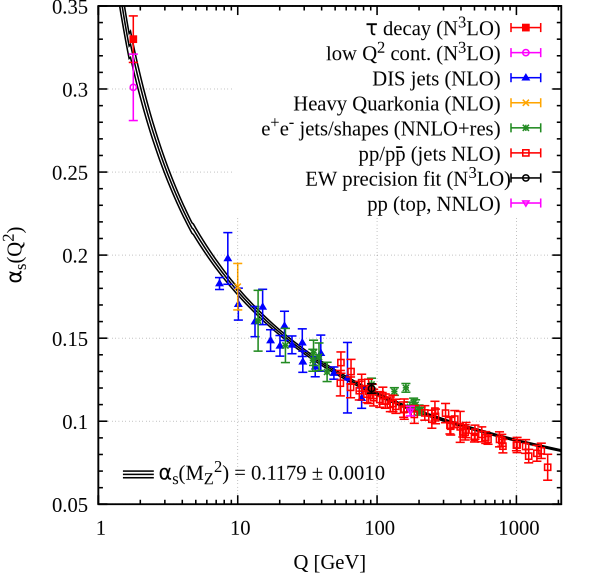
\includegraphics[width=.5\linewidth]{qcd}
 	\caption{Running coupling of QCD. The colored data points represent different methods to obtain a value for $\alpha_s$. For more details it may be referred to \cite{pdg}.}
 	\label{fig:coupl}
 \end{figure}

 For low ($<\SI{1}{\GeV}$) momentum transfers or large distances the coupling constant approaches infinity whereas it decreases for high ($\gg\SI{1}{\GeV}$) momentum transfers or short distances. These momentum ranges are referred to as \emph{confinement} and \emph{asymptotic freedom}, respectively; quarks are confined to remain in a bound state since if one tried to pull them apart the color field becomes so strong it will create a new quark anti-quark pair resulting in two new bound states. On the other hand, bound quarks behave quasi-free and can be described using perturbative quantum chromodynamics (pQCD) if probed at sufficiently large momentum transfers.

 It is more difficult however to describe QCD at momentum scales of $\approx \SI{1}{\GeV}$ since the coupling is too strong to justify a perturbative approach. Thus explicit modeling of QCD bound states is inevitable. One possibility is to describe baryons consisting of constituent quarks which are bound in a potential. Constituent quark models assume baryons are made up of three constituent quarks with effective masses differing from the bare quark mass. The effective mass is made up mostly from a sea of quark anti-quark pairs and gluons which surround the bare (valence) quarks. The explicit form of the binding potential is determined for each model.

 The Bonn model \cite{bonnmodel}, for example, is formulated as a relativistically covariant constituent quark model.
 A potential increasing linearly with the distance is employed to adequately describe confinement. The binding potential between the constituent quarks is described by an instanton-induced interaction. Baryon resonances are then states with an orbital or angular excitation of one of the quarks. Figure \ref{fig:bm} shows computed nucleon, that is Isospin $I=1/2$ resonances, of the Bonn model \cite{bonnmodel} on the left side of each column. These are compared to measured resonances and their PDG rating \cite{pdg} in the middle. Uncertainties are indicated by the colored areas. The resonances are identified by their total angular momentum and their parity $J\pi$. In addition also the total internal angular momentum along with isospin and again the total angular momentum $L_{2T2J}$ is given.
  \begin{figure}[htbp]
 	\centering
 	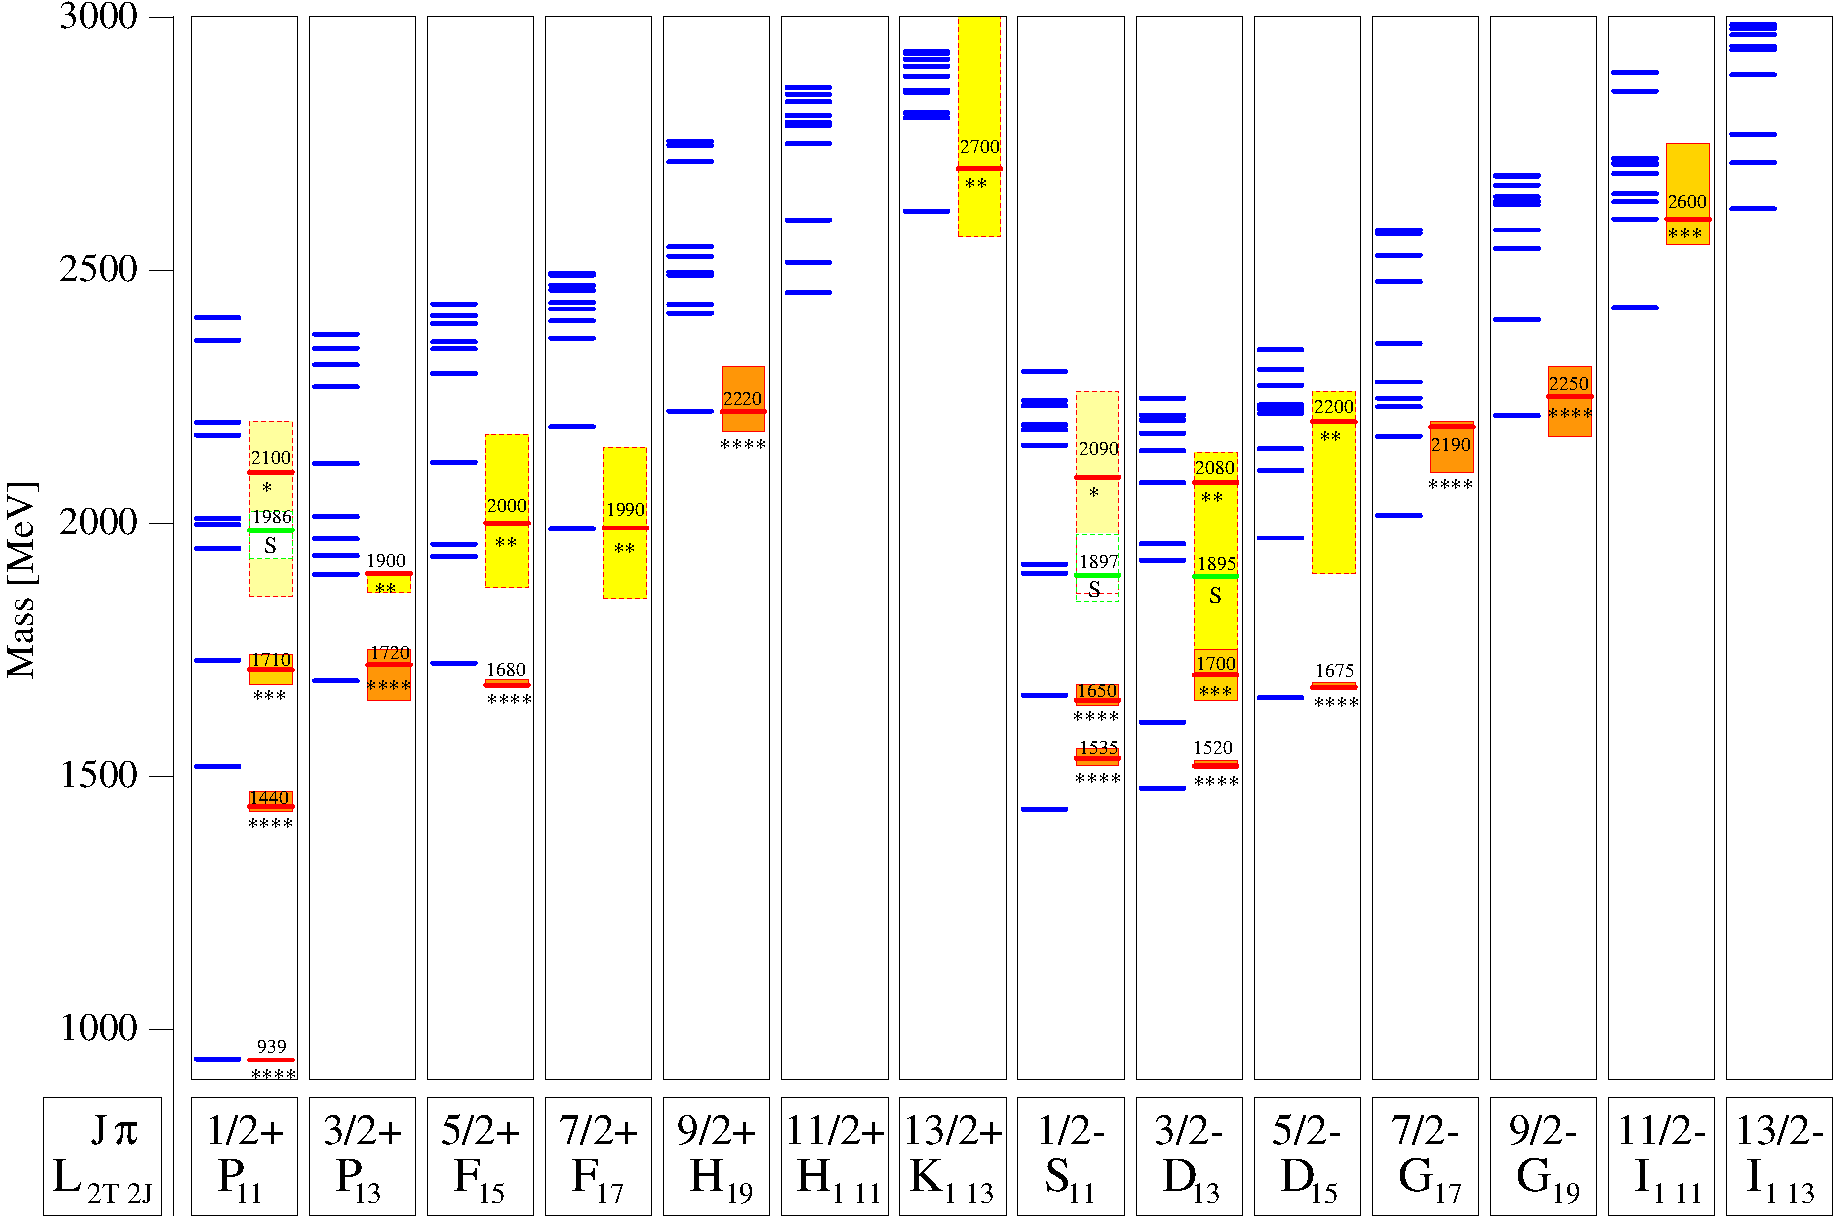
\includegraphics[width=\linewidth]{figs/NucM2.pdf}
 	\caption{Calculated nucleon (isospin $I=1/2$) resonances compared to measurements. Left in each column are the calculations \cite{bonnmodel}, the middle shows the measurements and PDG rating \cite{pdg}}
 	\label{fig:bm}
 \end{figure}
While generally good agreement exists for low lying resonances, especially for high masses there are much more resonances predicted than actually found. This is also known as the problem of the \enquote{missing resonances} indicating the poor understanding of QCD in the non-perturbative region. This can be due to several reasons: most of the knowledge about nucleon resonances and their properties was obtained investigating the $\pi N$ channel, biasing the data for resonances coupling weakly to this channel. Furthermore, the number of excited states with definite quantum numbers is related directly to the effective number of degrees-of-freedom accessible to the underlying theory. As a consequence, the number of degrees-of-freedom should be obtainable by comparing the measured states to the predicted states. Since nucleon resonances decay dominantly hadronic, their resonances are broad and overlapping. Thus on one hand the determination of excitation spectra proves to be a challenge on its own, demanding sophisticated methods, such as partial wave analysis (PWA). On the other hand it is not yet clear how many effective degrees-of-freedom exist for the nucleon in a constituent quark model. They could for example be decreased if the nucleon were made up of a quark and a di-quark structure. In either case it should prove fruitful to investigate the photoproduction of mesons off the nucleon for different final states to access the resonances and transitions between them which are of interest. This should ultimately add to the understanding of QCD in the non-perturbative regime. \cite{Krusche}


\section{Photoproduction of Pseudoscalar Mesons}
From the scattering theory point of view, photoproduction of mesons is well understood \cite{Krusche}. Figure \ref{fig:mes_bildchen} shows schematically the process thereof off the proton:

\begin{figure}[htbp]
	\centering
	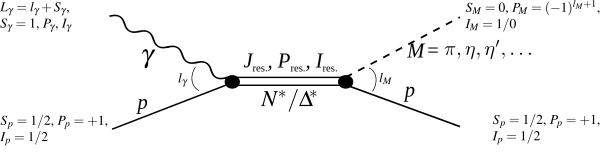
\includegraphics[width=\linewidth]{meson_bildchen}
	\caption{\textsc{Feynman} diagram for the s-channel photoproduction of pseudoscalar mesons, adapted from \cite{farahphd}}
	\label{fig:mes_bildchen}
\end{figure}

The analysis requires partial wave decomposition in both initial and final states \cite{Drechsel} since the intermediate resonance has definite angular momentum, parity  and isospin $J_\text{res.}, P_\text{res.}, I_\text{res.}$. The resonance is excited by a photon with (iso-) spin $I_\gamma,S_\gamma =1$ and parity $P_\gamma$ coupling electromagnetically to the target proton with (iso-) spin $I_p=1/2,S_p=1/2$ and parity $P_p$. The relative momentum is $l_\gamma$, such that the total momentum of the photon is $L_\gamma=l_\gamma+S_\gamma$. Subsequently the intermediate state will have the quantum numbers $J_\text{res.}, P_\text{res.}, I_\text{res.}$ and decay into a pseudoscalar ($S_M=0$) meson with isospin $I_M$, relative orbital angular momentum $l_M$ und Parity $P_M=(-1)^{l_M+1}$ and a proton. The following selection rules can be derived using parity and momentum conservation \cite{Krusche,farahphd}
\begin{align}
	%\left|L_\gamma-S_p\right|&=\left|L_\gamma-1/2\right|\leq J_\text{res.}\leq\left|L_\gamma+1/2\right|=\left|L_\gamma+S_p\right|,\\
	J_\text{res.}&=L_\gamma\oplus S_p = L_\gamma\oplus 1/2,\\
	P_\text{res.}&=P_p\cdot P_\gamma=P_\gamma,\\
	%\left|l_M-S_p\right|&=\left|l_M-1/2\right|\leq J_\text{res.}\leq\left|l_M+1/2\right|=\left|l_M+S_p\right|,\\
	J_\text{res.}&=l_M\oplus S_p = l_M\oplus 1/2\\
	P_\text{res.}&=P_p\cdot P_M=(-1)^{l_M+1},
\end{align}
where the usual rules for the coupling of angular momenta \cite{theo3} apply. Thus, knowledge of the photoproduction multipoles allows the identification of contributing resonances for particular mesonic final states. Table \ref{tab:qn} shows relevant resonances for the lowest order of photon multipoles ($L_\gamma=1$).

\begin{table}[htbp]
	\begin{tabular}{cccccc}
		\toprule
		E
	\end{tabular}
\caption{Allowed quantum numbers for the intermediate resonance state $N^*/\Delta^*$}
\label{tab:qn}
\end{table}

\section{Measurement of Polarization Observables}

\section{Introduction to \textsc{Bayesian} statistics}

\section{Motivation and Structure of this Thesis}
bla

% !TEX root = master_thesis.tex
\chapter{Experimental Setup}
As motivated in the previous chapter, it is promising to study the photoproduction of pseudoscalar mesons in order to determine a complete set of polarization observables. This requires a polarized photon beam and/or a polarized target. It is convenient to study photoproduction off a fixed target and investigate the resonances that occur in the process. Incidentally, these resonances can only be accessed via their decay products, such that suitable calorimeters are needed. The CBELSA/TAPS experiment is  located in Bonn  at the ELectron Stretcher Accelerator (ELSA), which can be used to generate a high energy photon beam using the \emph{bremsstrahlung} process, meets all above mentioned requirements. This chapter will elaborate on the already mentioned parts of the experiment that was used to collect the data needed for the determination of the target asymmetry in $\eta'$ photoproduction.

\section{Production of (polarized) high energy photon beam}
First of all, a high energy photon beam has to be produced.
\begin{figure}[htbp]
	\centering
	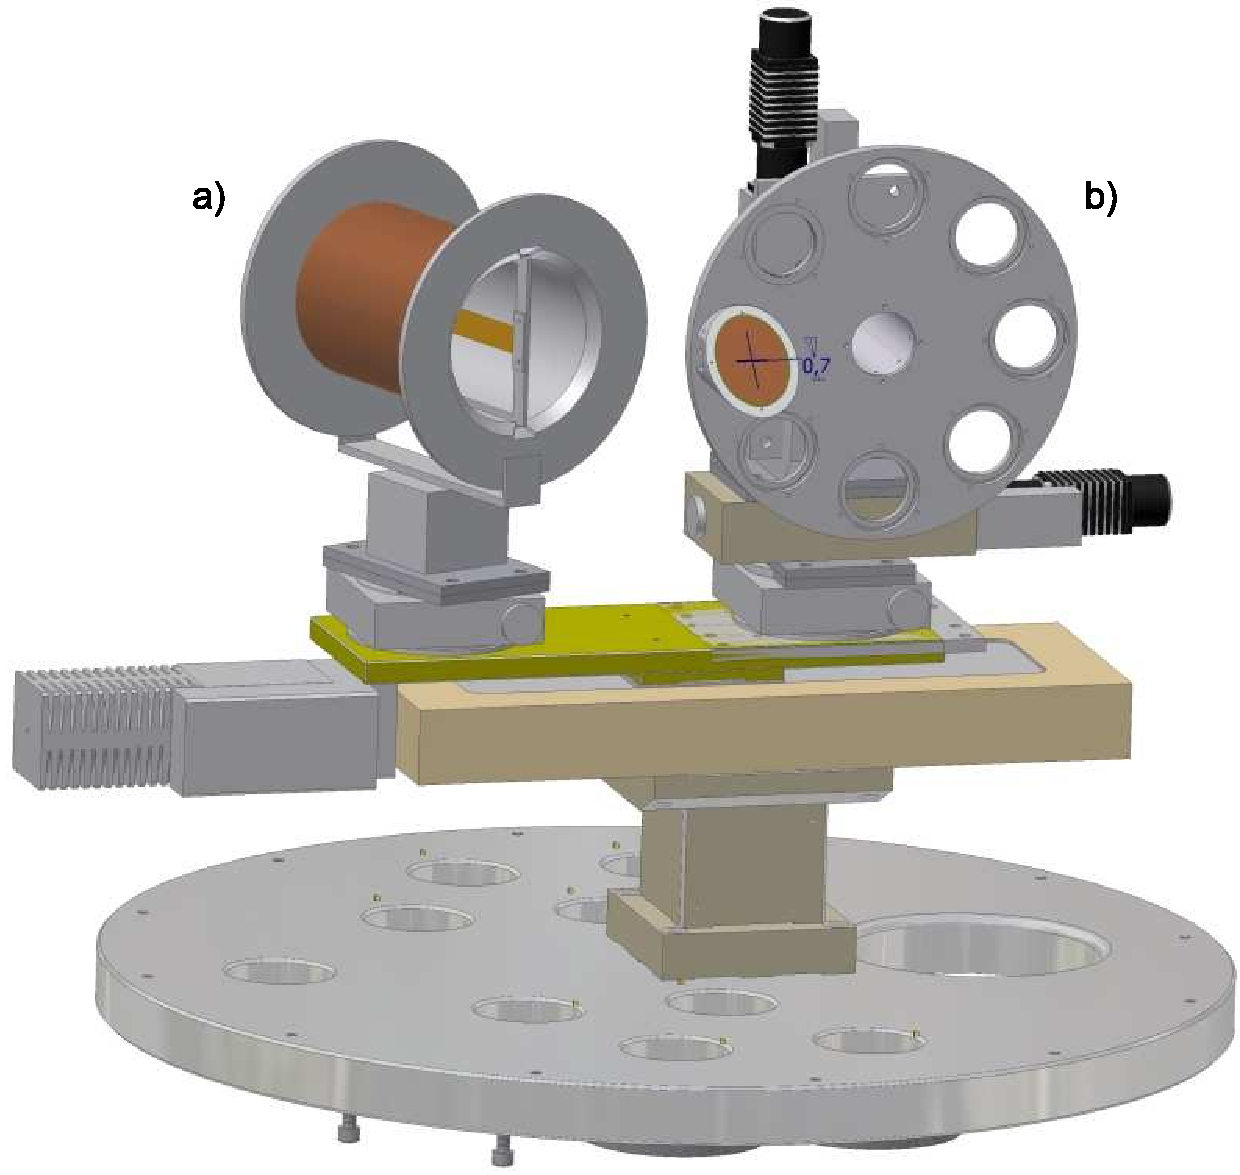
\includegraphics[width=.49\linewidth]{figs/goni-ganz.pdf}
	\caption{\cite{cb}}
\end{figure}
\begin{figure}[htbp]
	\centering
	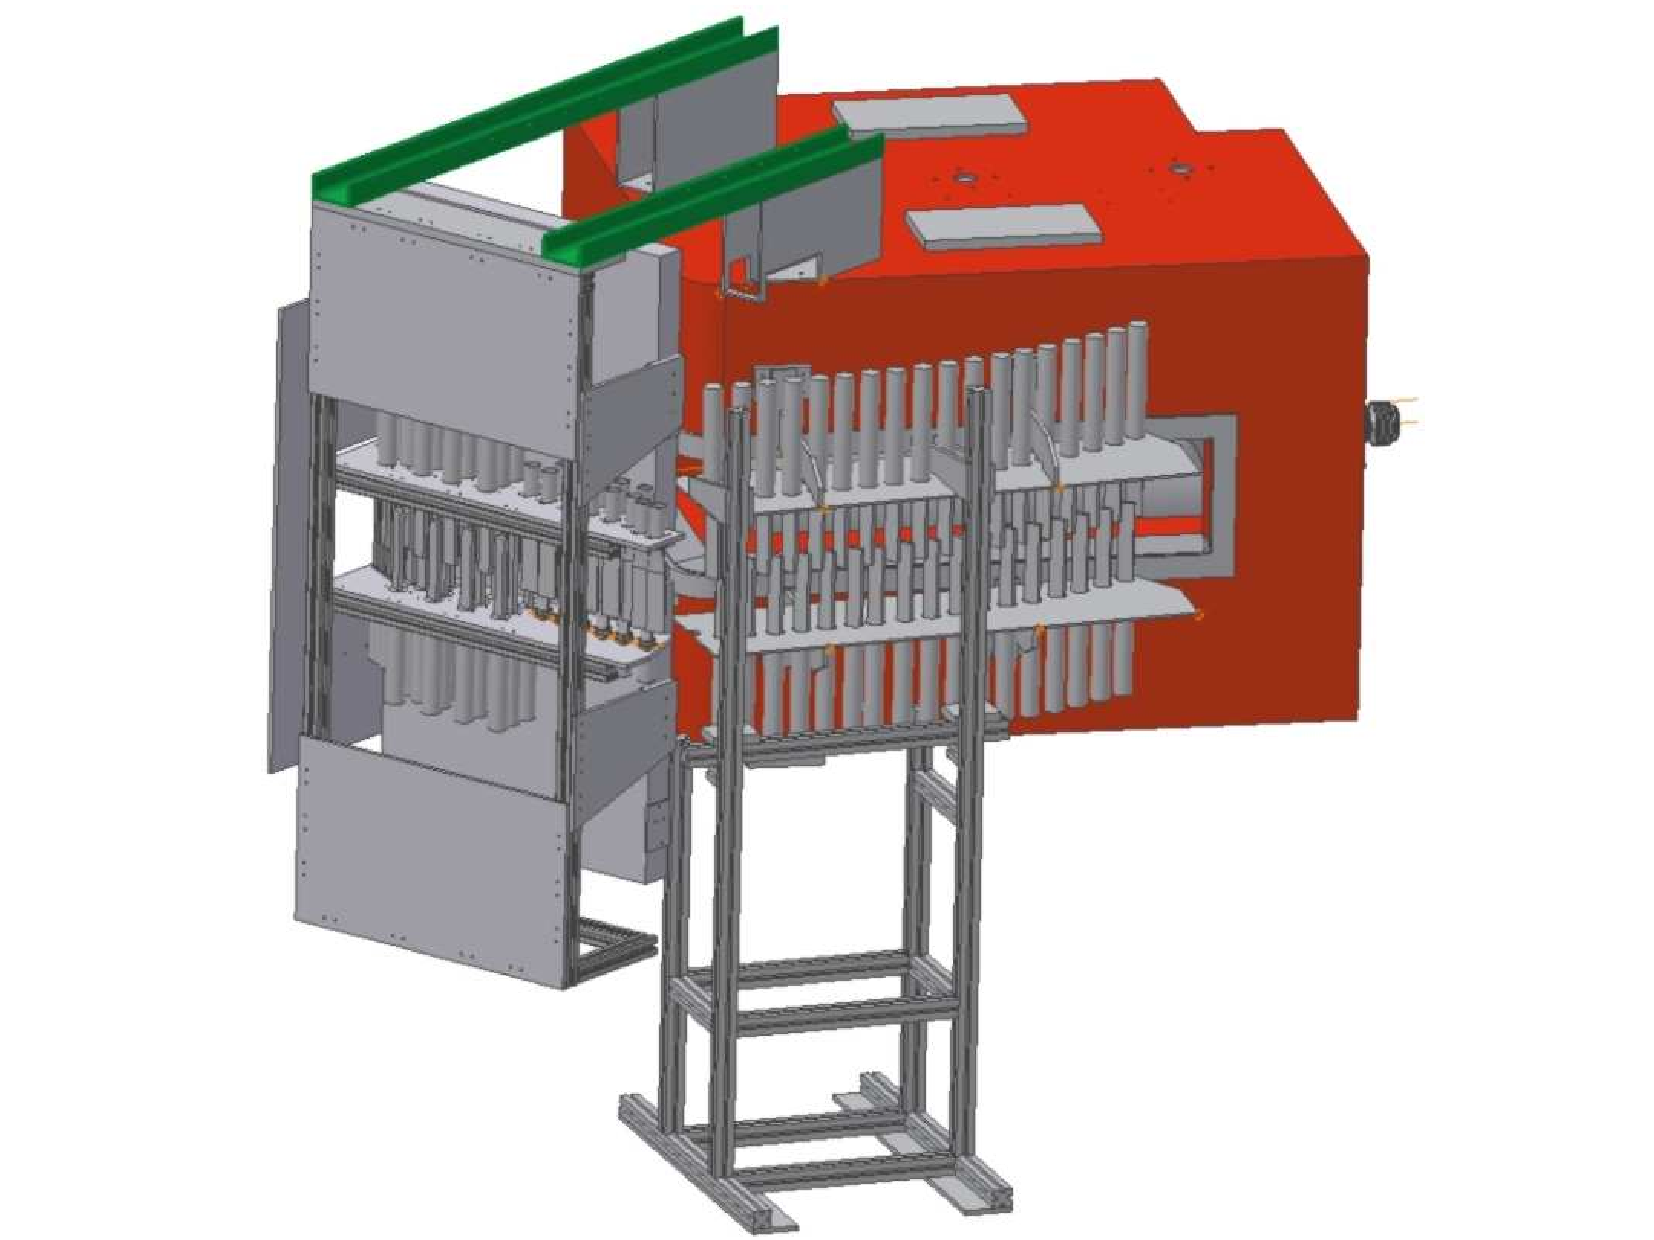
\includegraphics[width=.49\linewidth]{figs/Tagger.pdf}
	\caption{\cite{cb}}
\end{figure}
\subsection{Tagger}
\label{subsec:tag}
\section{Beam Target}

\begin{figure}[htbp]
	\centering
	\includegraphics[width=.5\linewidth]{figs/Target.pdf}
	\caption{\cite{cb}}
\end{figure}
\section{Calorimeters}
\begin{figure}[htbp]
	\centering
	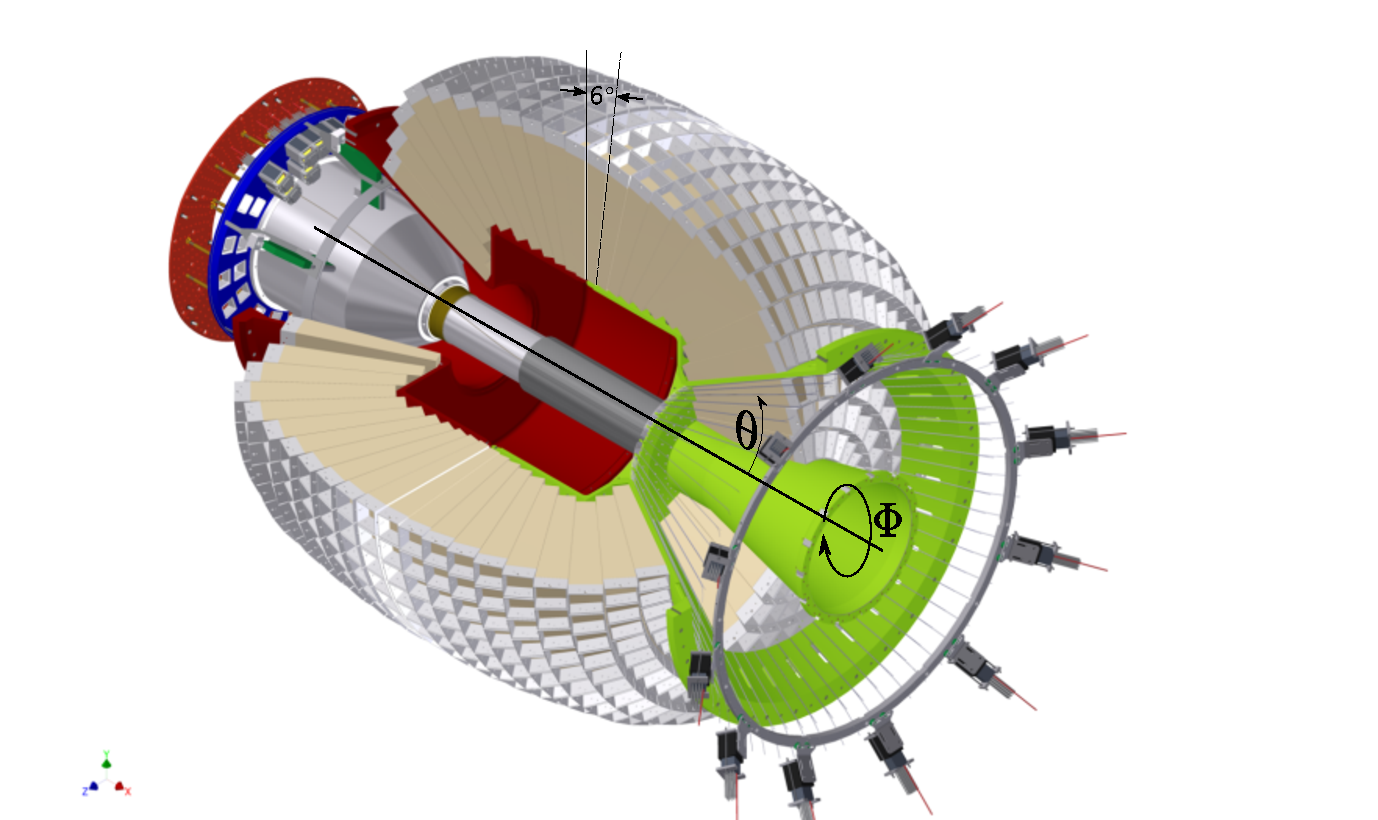
\includegraphics[width=\linewidth]{figs/cb_fp_in.pdf}
	\caption{\textsc{D. Walther} in \cite{urban}}
\end{figure}
\begin{figure}[htbp]
	\centering
	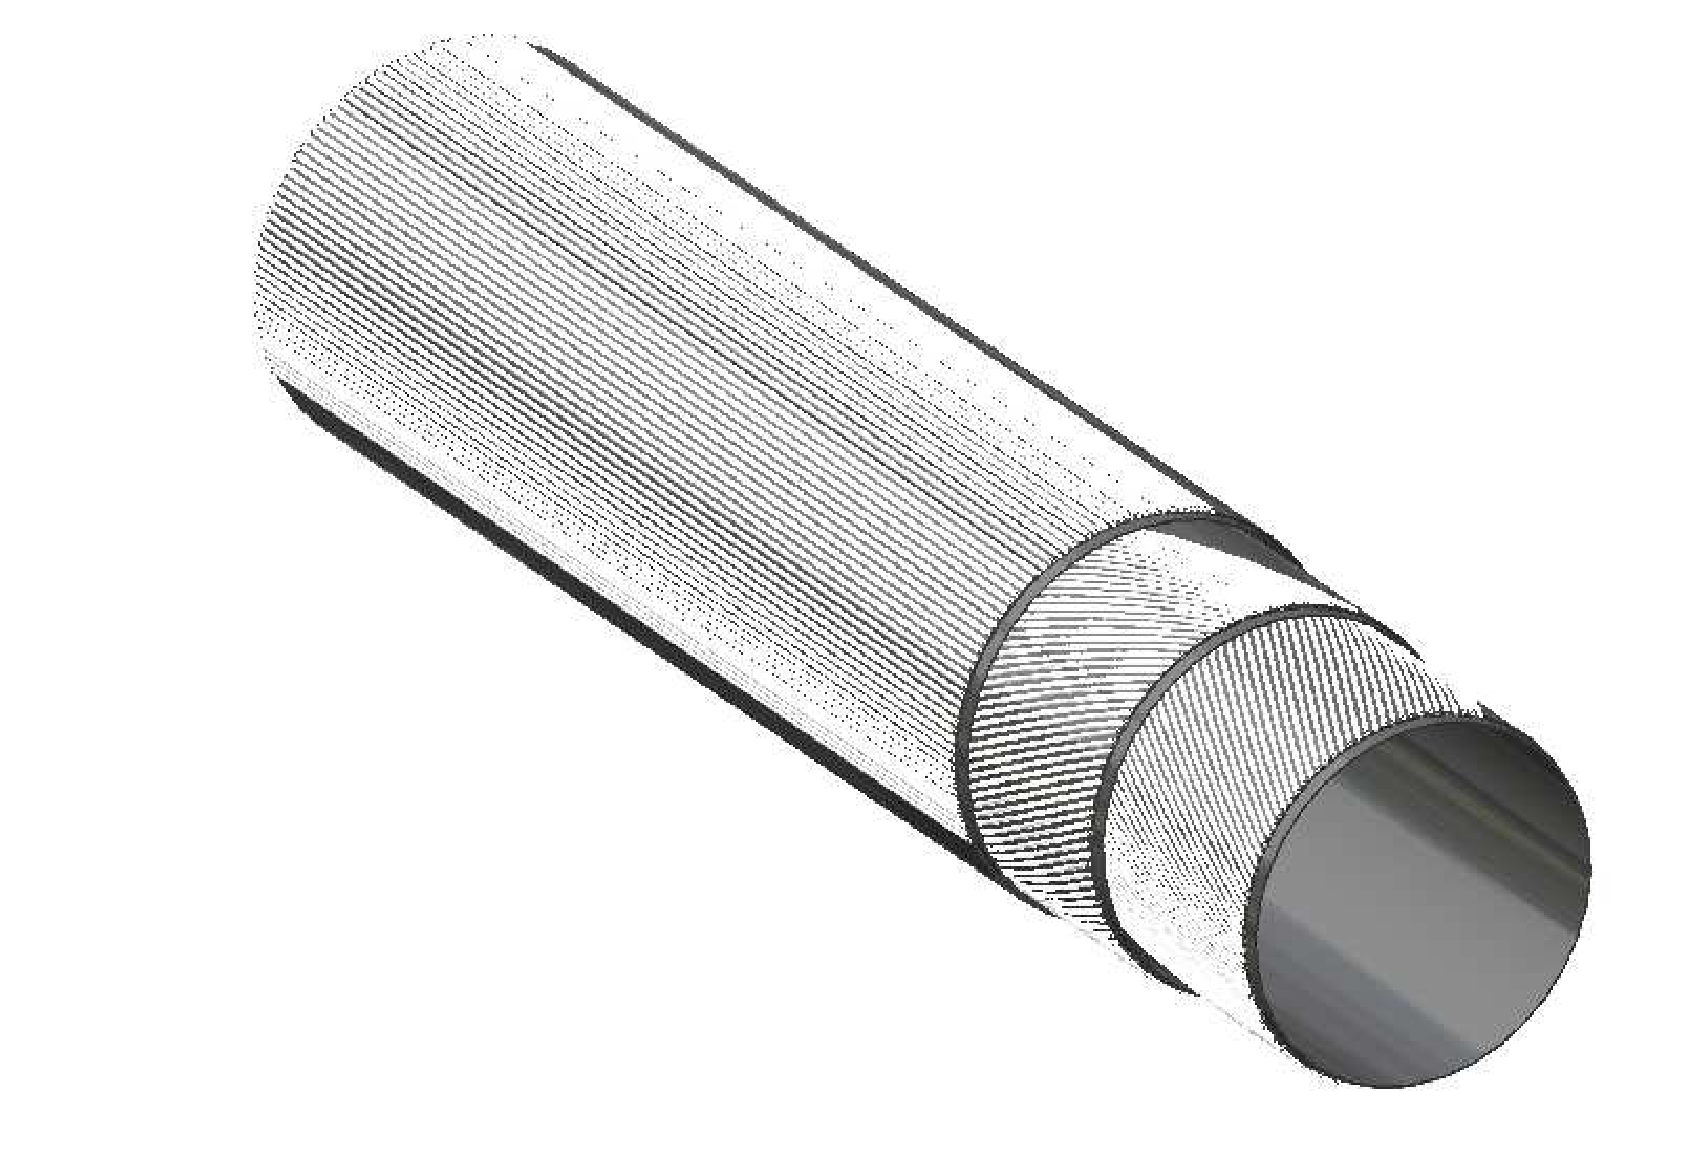
\includegraphics[width=.5\linewidth]{figs/faserorient.pdf}
	\caption{\cite{cb}}
\end{figure}
\begin{figure}[htbp]
	\centering
	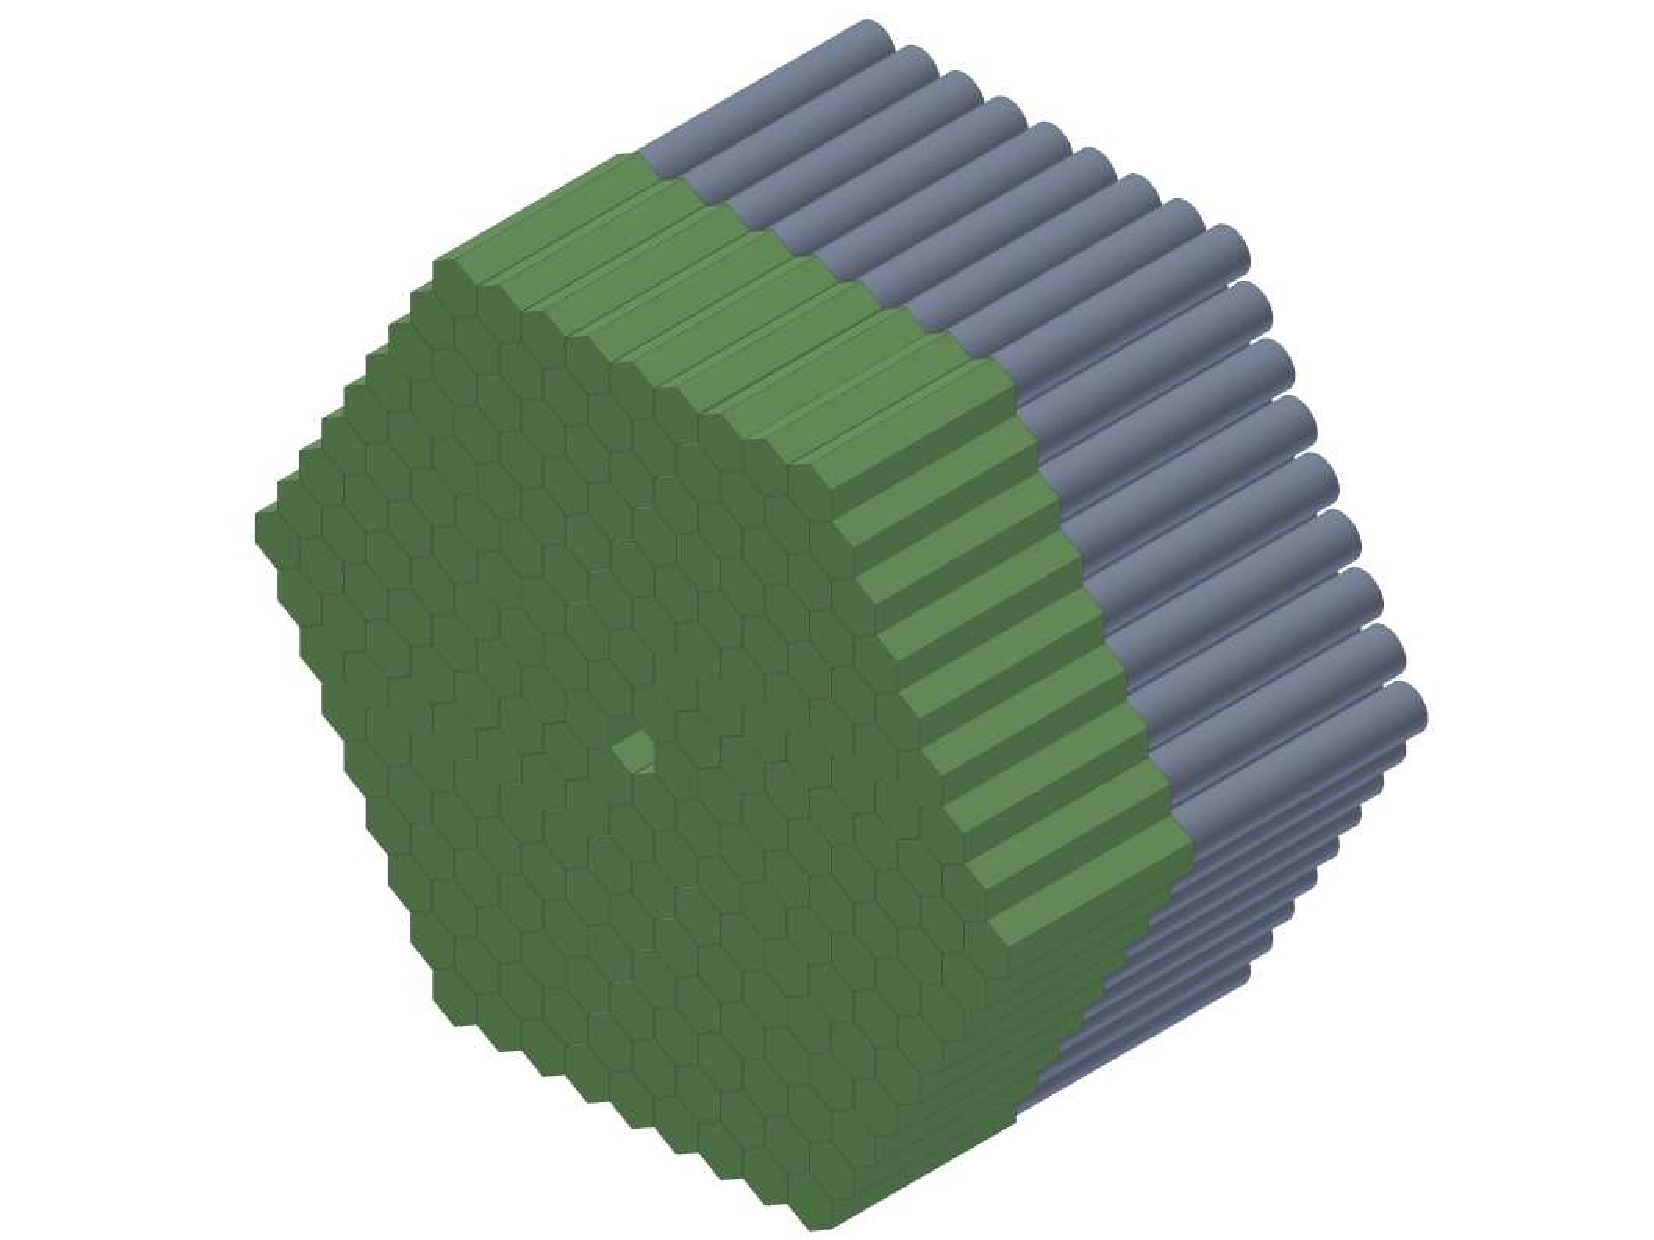
\includegraphics[width=.5\linewidth]{figs/mini-taps.pdf}
	\caption{\cite{cb}}
\end{figure}

\section{Trigger}
% Uncomment the following command to get references per chapter.
% Put it inside the file or change \include to \input if you do not want the references
% on a separate page
% \printbibliography[heading=subbibliography]

%------------------------------------------------------------------------------
% Include the following lines and comment out \printbibliography if
% you use BiBTeX for the bibliography.
% If you use biblatex package the files should be specified in the preamble.
% \KOMAoptions{toc=bibliography}
% {\raggedright
%   \bibliographystyle{../refs/atlasBibStyleWithTitle.bst}
%   % \bibliographystyle{unsrt}
%   \bibliography{./thesis_refs,../refs/standard_refs-bibtex}
% }

%------------------------------------------------------------------------------
\appendix
% \part*{Appendix}
% Add your appendices here - don't forget to also add them to \includeonly above
%------------------------------------------------------------------------------
\chapter{Illustration of used software tools}
\label{app:soft}
\section{ExPLORA}
Figure \ref{fig:xml} shows an example of a \texttt{.xml} file that was used to call the plugin that was written to select the reaction $\gamma p\to p\eta'\to p\gamma\gamma$. First of all, several files have to be included in order to acquire certain \emph{containers} that inhibit the raw data of the final state particles. Then the plugin is embedded with the options 
\begin{itemize}
	\item \texttt{MC} (bool) -- determines whether Monte Carlo or measured data are analyzed 
	\item \texttt{PWA} (bool) -- determines whether used Monte Carlo simulation have PWA weights
	\item \texttt{FOURGAMMAS} (bool) -- determines whether the generated final state has four photons or two
	\item \texttt{REALGAMMAS} (bool) -- determines whether real photons are part of the decay or not (e.g. $n\pi^+$)
	\item \texttt{allroutes} (CBTConfigString) -- gives the container that contains the routes of charged particles
\end{itemize}
\begin{figure}[htbp]
	\centering
	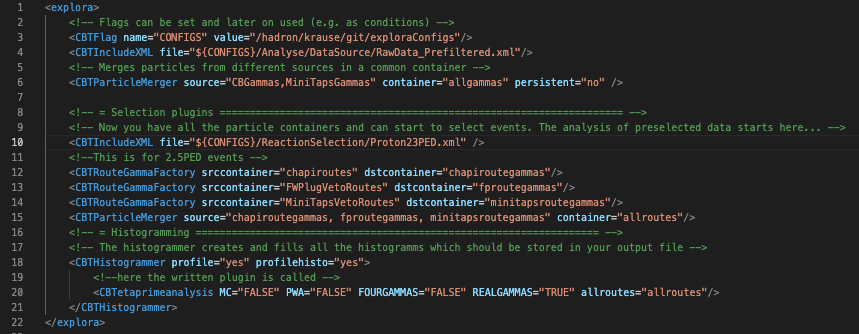
\includegraphics[width=\linewidth]{../demonstration/new_gg.png}
	\caption{Example \texttt{.xml} file that was used to call the plugin \texttt{CBTetaprimeanalysis.cpp} (line 20) with several self defined options.}
	\label{fig:xml}
\end{figure}
\section{Stan}
In chapter \ref{chap:intro} an example fit using \emph{Stan} was shown. Data was fitted that followed a cosine distribution
\begin{equation}
	y=a\cdot \cos x +b+\epsilon.
\end{equation}
Here $y$ is a measured quantity with \textsc{Gaussian} noise $\epsilon$, $x$ are predictors and $a$ and $b$ are fit parameters. Assuming each datapoint $y_n$ is independent and exhibits an individual noise term $\epsilon_n\sim\mathcal{N}(0,\sigma_n)$, the likelihood $p(y|a,b)$ can be formulated as
\begin{align}
	y_n\sim\mathcal{N}(a\cdot\cos(x_n) +b,\sigma_n)&&\Leftrightarrow& &p(y|a,b)=\prod_{i=1}^N\mathcal{N}(y_n|a\cdot\cos(x_n)+b,\sigma_n),
\end{align} 
if there are $N$ datapoints in total. Specifying e.g. normal priors for the two regression coefficients $a$ and $b$ completes the inference
\begin{align}
	a\sim\mathcal{N}(0,1)&&b\sim\mathcal{N}(0,1).
\end{align}
Figure \ref{fig:stan} shows the implementation of the described model in \emph{Stan}. First of all, all data that is read in has to be defined. Conveniently this can be done using the \texttt{vector} class, that corresponds to a list of e.g. all $x$ values. Next, the parameters of the model are defined and the likelihood and priors are specified. Samples from the posterior predictive distribution are randomly sampled using all simulation draws in a last step.
\begin{figure}[htbp]
	\centering
	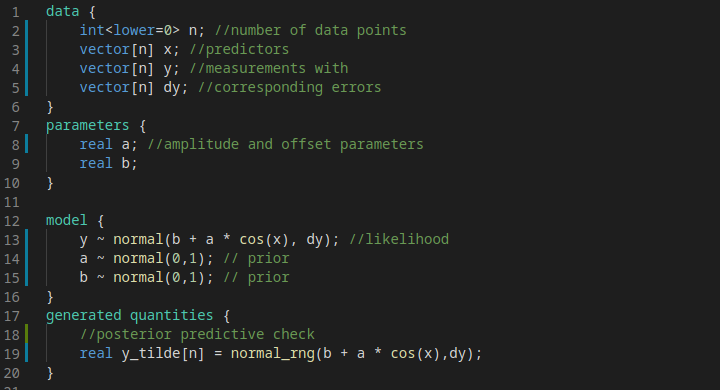
\includegraphics[width=\linewidth]{../demonstration/stanfile.png}
	\caption{Example \texttt{.stan} file that can be used to perform a simple linear fit.}
	\label{fig:stan}
\end{figure}
\chapter{Additional plots and calculations}
\label{sec:app}
%------------------------------------------------------------------------------
This chapter will give additional calculations and plots which would have interrupted the train of thought unnecessarily in the main part. 
\section{Statistical error for the asymmetry $A(\phi)$}
\allowdisplaybreaks
\label{sec:stat_err}
Let $\tilde{N}^{\parallel/\bot}_i$ be the normalized event yields at bin $\phi_i$. As mentioned in section \ref{sec:meth}, the asymmetry $A_i$ at bin $i$ is then given by
\begin{equation}
	A_i=\frac{\tilde{N}^\bot_i-\tilde{N}^\parallel_i}{p_\gamma^\parallel\tilde{N}^\bot_i+p_\gamma^\bot\tilde{N}^\parallel_i}=\Sigma\cos\left(2\left(\alpha^\parallel-\phi_i\right)\right),
	\label{eq:evyieldasym_app}
\end{equation}
where the event yields are normalized over all $M$ $\phi$-bins $$\tilde{N}^{\parallel/\bot}_i=\frac{N_i^{\parallel/\bot}}{\sum_{j=1}^{M}N_j^{\parallel/\bot}}.$$
 To estimate statistical errors according to \textsc{Gaussian} error propagation, the partial derivatives with respect to $\tilde{N}_i^{\parallel/\bot}$ have to be built:
 \begin{equation}
 	\left(\Delta A_i\right)^2=\left(\frac{\partial A_i}{\partial \tilde{N}^\parallel_i}\Delta \tilde{N}^\parallel_i\right)^2+\left(\frac{\partial A_i}{\partial \tilde{N}^\bot_i}\Delta \tilde{N}^\bot_i\right)^2,
 \end{equation}
where
\begin{align}
	\left(\frac{\partial A_i}{\partial \tilde{N}^{\parallel/\bot}_i}\right)^2&=\left[\frac{\tilde{N}^{\bot/\parallel}_i\left(p_\gamma^\bot+p_\gamma^\parallel\right)}{\left(p_\gamma^\parallel\tilde{N}^{\bot}_i+p_\gamma^\bot\tilde{N}^\parallel_i\right)^2}\right]^2,\\
	&\text{ and with } \tilde{N}_i^{\bot/\parallel}=\tilde{N}_i\\
	\left(\Delta\tilde{N}_i\right)^2&=\left[\frac{\partial}{\partial N_i}\left(\frac{N_i}{\sum_{j}N_j}\right)\cdot\Delta N_i\right]^2+\sum_{j\neq i}\left[\frac{\partial}{\partial N_j}\left(\frac{N_i}{\sum_{j}N_j}\right)\cdot\Delta N_j\right]^2\\
	&=\left[\frac{\sum_{j\neq i} N_j}{\left(\sum_{j} N_j\right)^2}\cdot\Delta N_i\right]^2+\sum_{j\neq i}\left[-1\cdot\frac{N_i}{\left(\sum_{j}N_j\right)^2}\cdot\Delta N_j\right]^2\\
	&=\frac{1}{\left(\sum_{j} N_j\right)^4}\cdot\left[\left(\sum_{j\neq i} N_j \cdot\Delta N_i\right)^2+\sum_{j\neq i}\left(N_i\cdot\Delta N_j\right)^2\right].
\end{align}
One can then further use that $\left(\Delta N_i\right)^2  \approx N_i$. This holds only approximately, since the histograms are filled $N$ times with weights $w_n$ (see chapter \ref{sec:time}), but since the weights are either $w=1$ or $w\ll1$
\begin{equation}
	\Delta N_i=\sqrt{\sum_{n=1}^N w^2}\approx\sqrt{N_i}.
\end{equation}
\newpage
\section{Kinematic variables for each bin}
\label{sec:kinv}
\subsection{Coplanarity}
\begin{figure}[H]
	\centering
	\begin{subfigure}{\linewidth}
		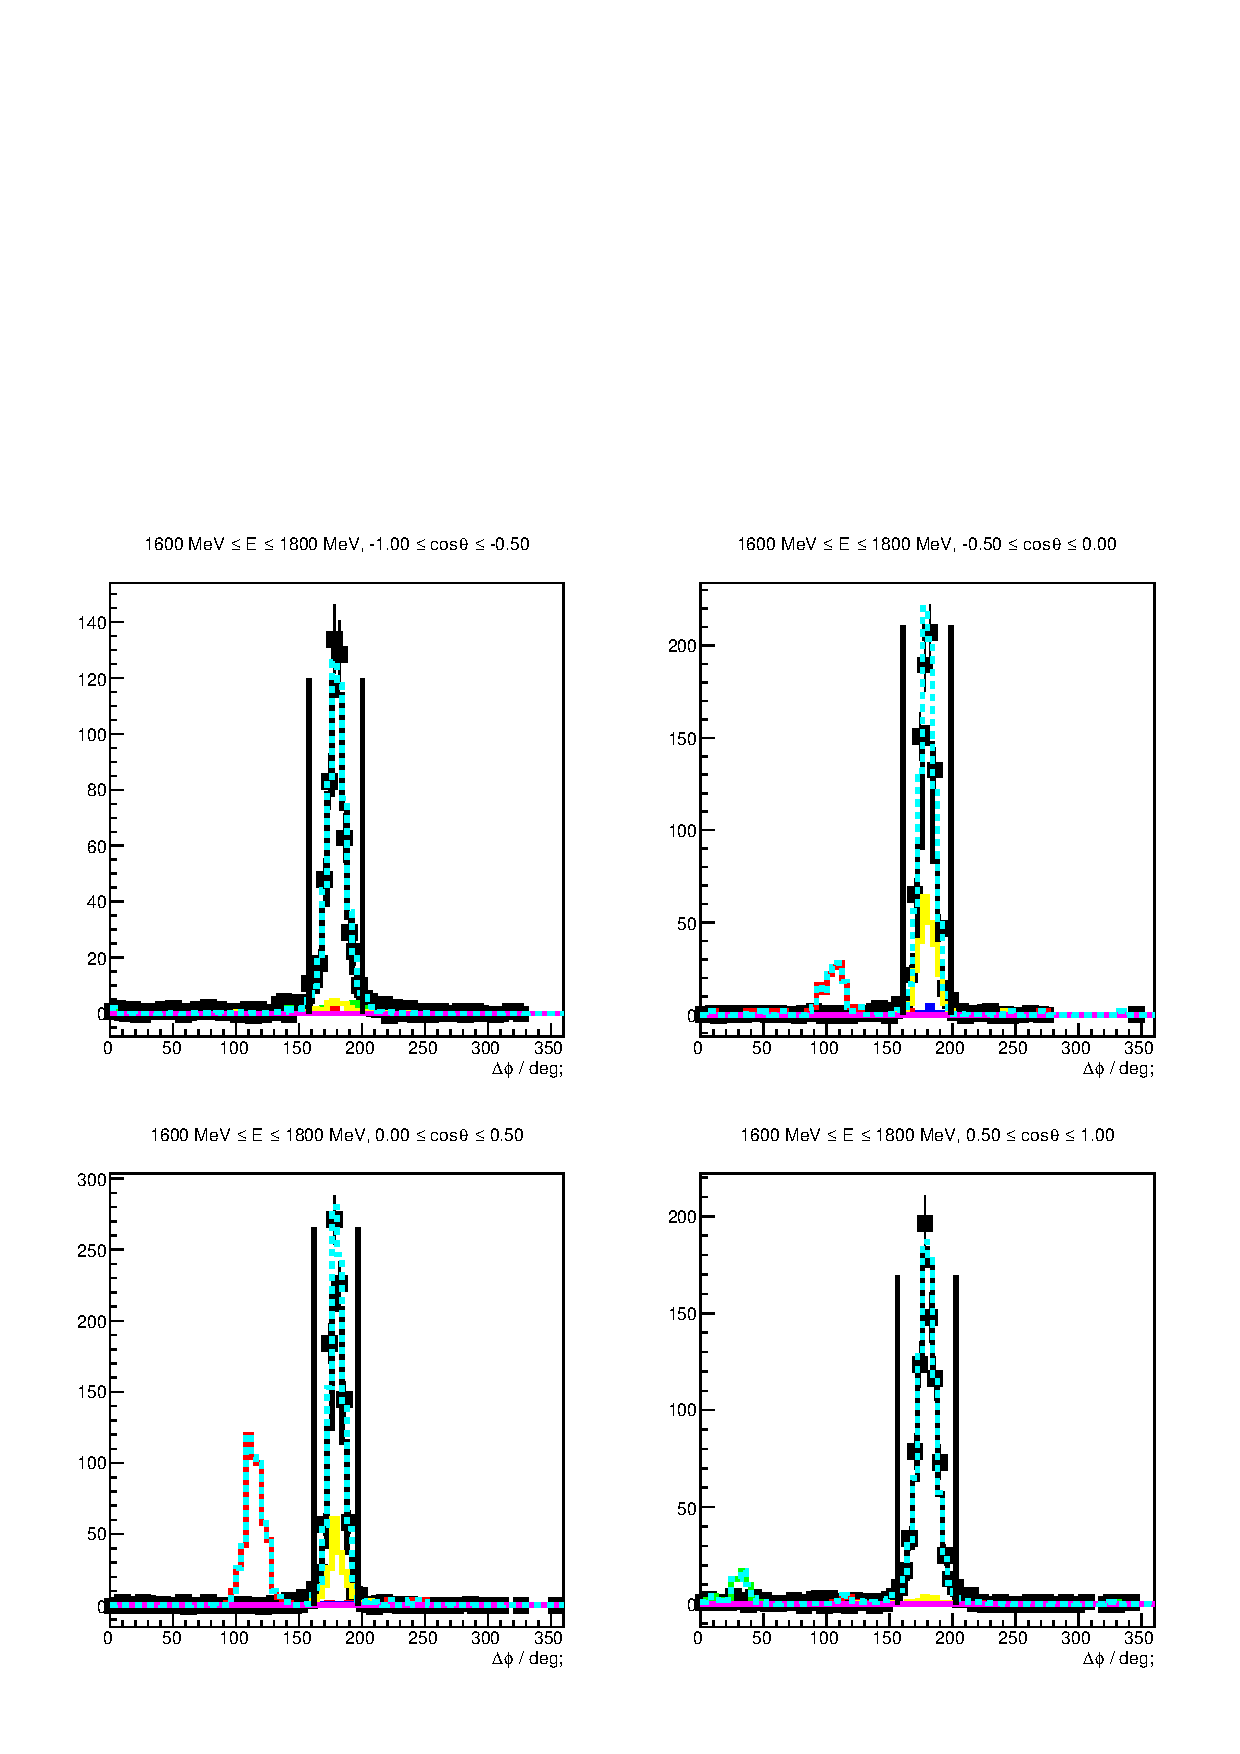
\includegraphics[width=\linewidth]{../figs/hydrogen/bin_cuts/phicut_ebin1.pdf}
		\subcaption{$\SI{1500}{\mega\eV}\leq E_\gamma<\SI{1600}{\mega\eV}$}
	\end{subfigure}

	\begin{subfigure}{\linewidth}
		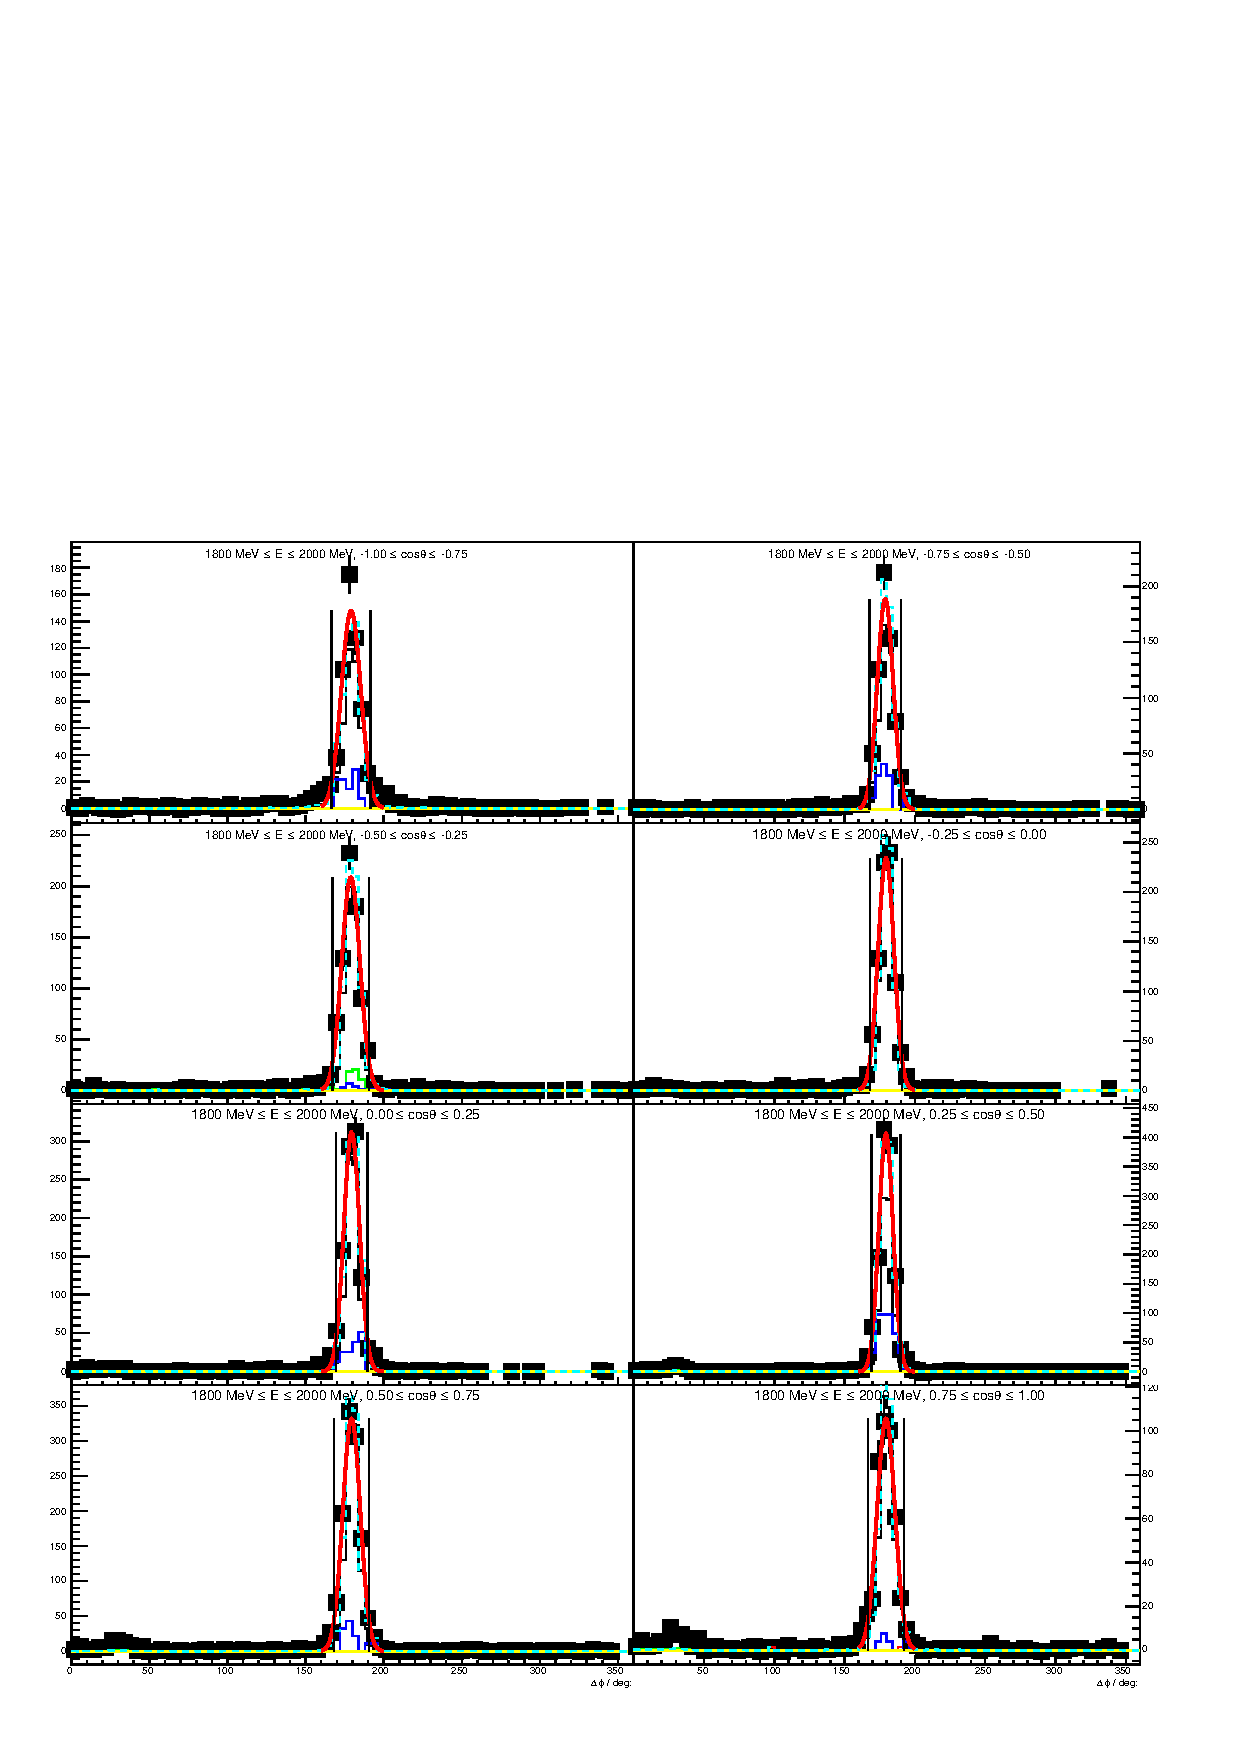
\includegraphics[width=\linewidth]{../figs/hydrogen/bin_cuts/phicut_ebin2.pdf}
		\subcaption{$\SI{1600}{\mega\eV}\leq E_\gamma<\SI{1700}{\mega\eV}$}
	\end{subfigure}
\caption{Coplanarity $\Delta\phi$ for all energy and angular bins. Data points are displayed as open circles, scaled Monte Carlo data belonging to $\eta'$ photoproduction is displayed as solid histogram. The determined cut ranges are indicated by the dashed red lines.}
\end{figure}
\begin{figure}[H]
\ContinuedFloat
	\begin{subfigure}{\linewidth}
		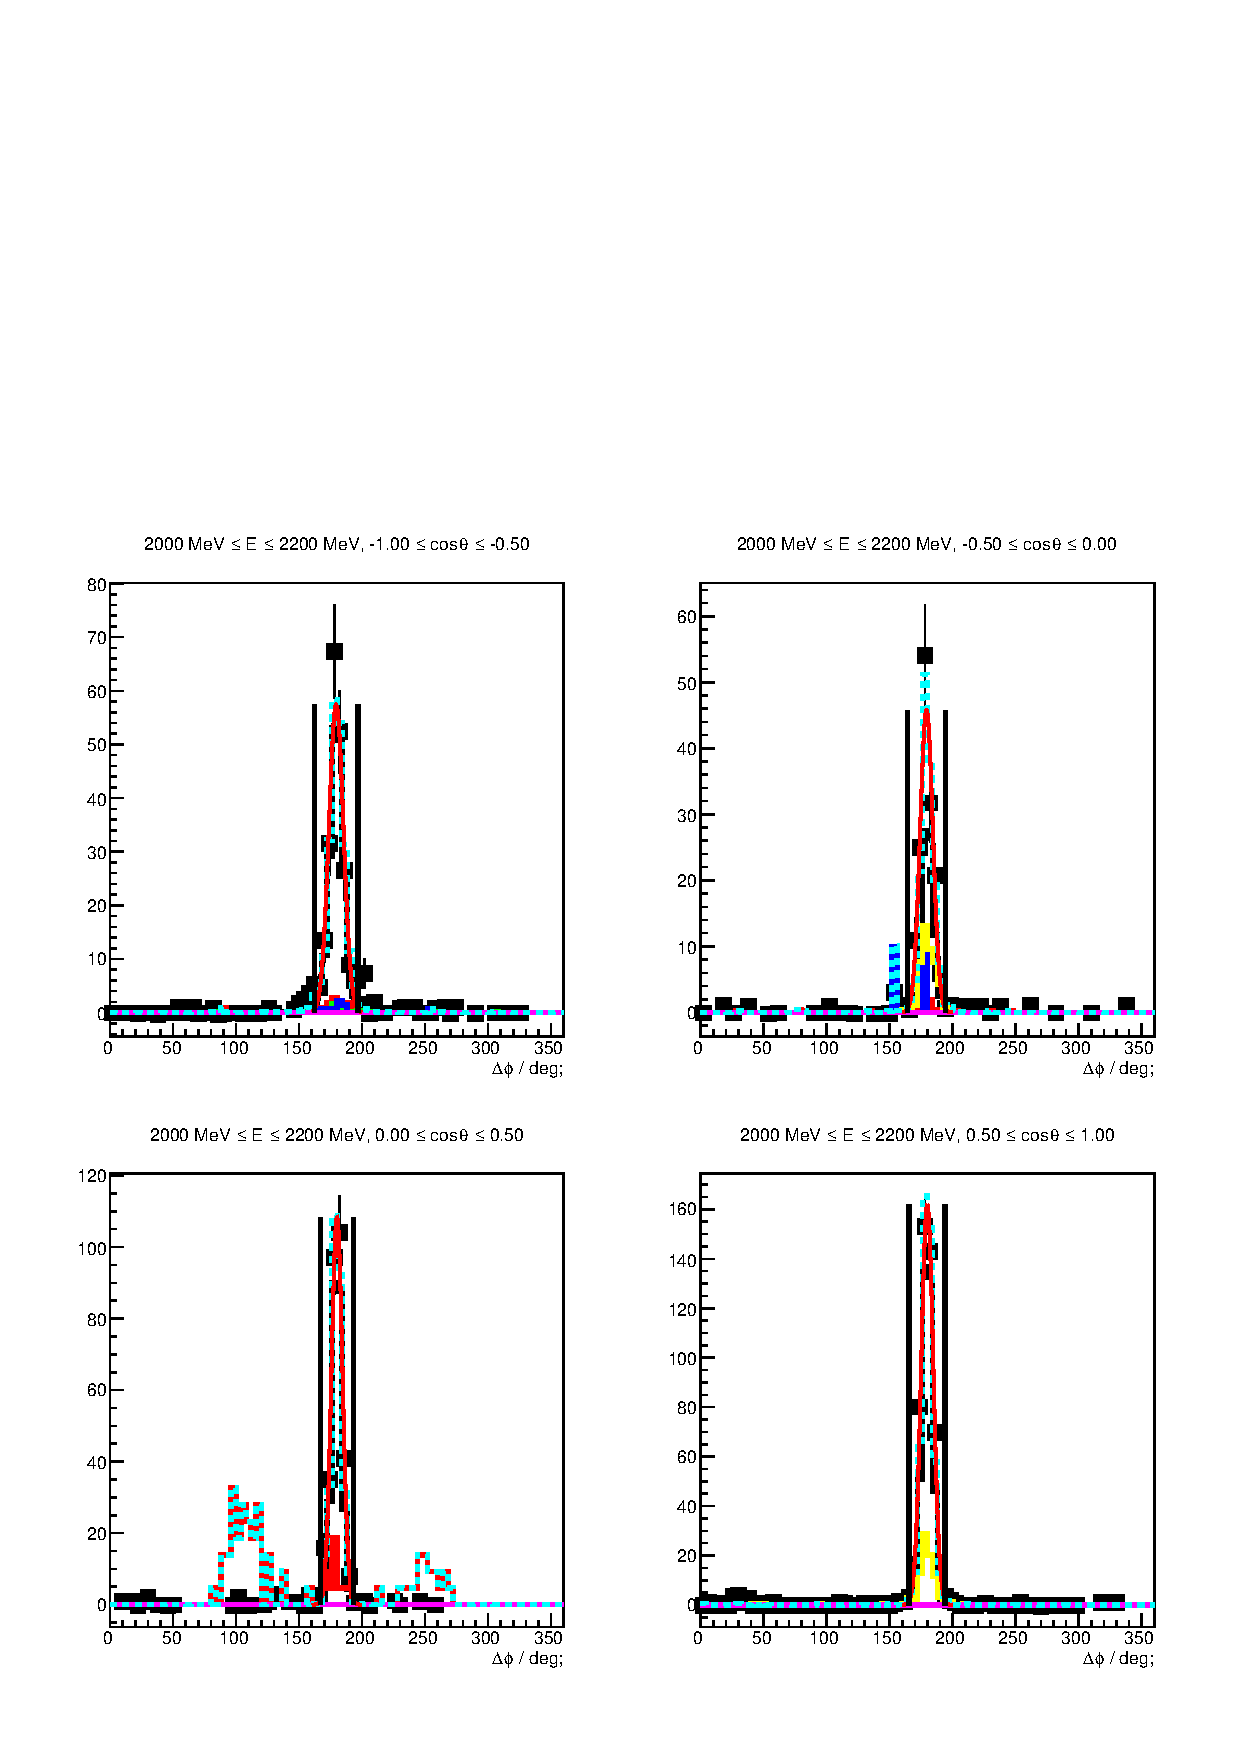
\includegraphics[width=\linewidth]{../figs/hydrogen/bin_cuts/phicut_ebin3.pdf}
		\subcaption{$\SI{1700}{\mega\eV}\leq E_\gamma<\SI{1800}{\mega\eV}$}
	\end{subfigure}
\caption{Coplanarity $\Delta\phi$ for all energy and angular bins. Data points are displayed as open circles, scaled Monte Carlo data belonging to $\eta'$ photoproduction is displayed as solid histogram. The determined cut ranges are indicated by the dashed red lines.}
\label{fig:appcopl}	
\end{figure}
Figure \ref{fig:appcopl} shows the coplanarity for all energy and angular bins. Cut ranges were determined from a \textsc{Gaussian} fit to the data points. Only slight dependency on beam energy and meson polar angle can be identified. Only $\eta'$ Monte Carlo data are fitted because the measured points do not give enough reference points for the fit to identify different contributing final states. There is good agreement between Monte Carlo simulations and measured data.
\newpage
\subsection{Polar angle difference}
\begin{figure}[H]
	\centering
	\begin{subfigure}{\linewidth}
		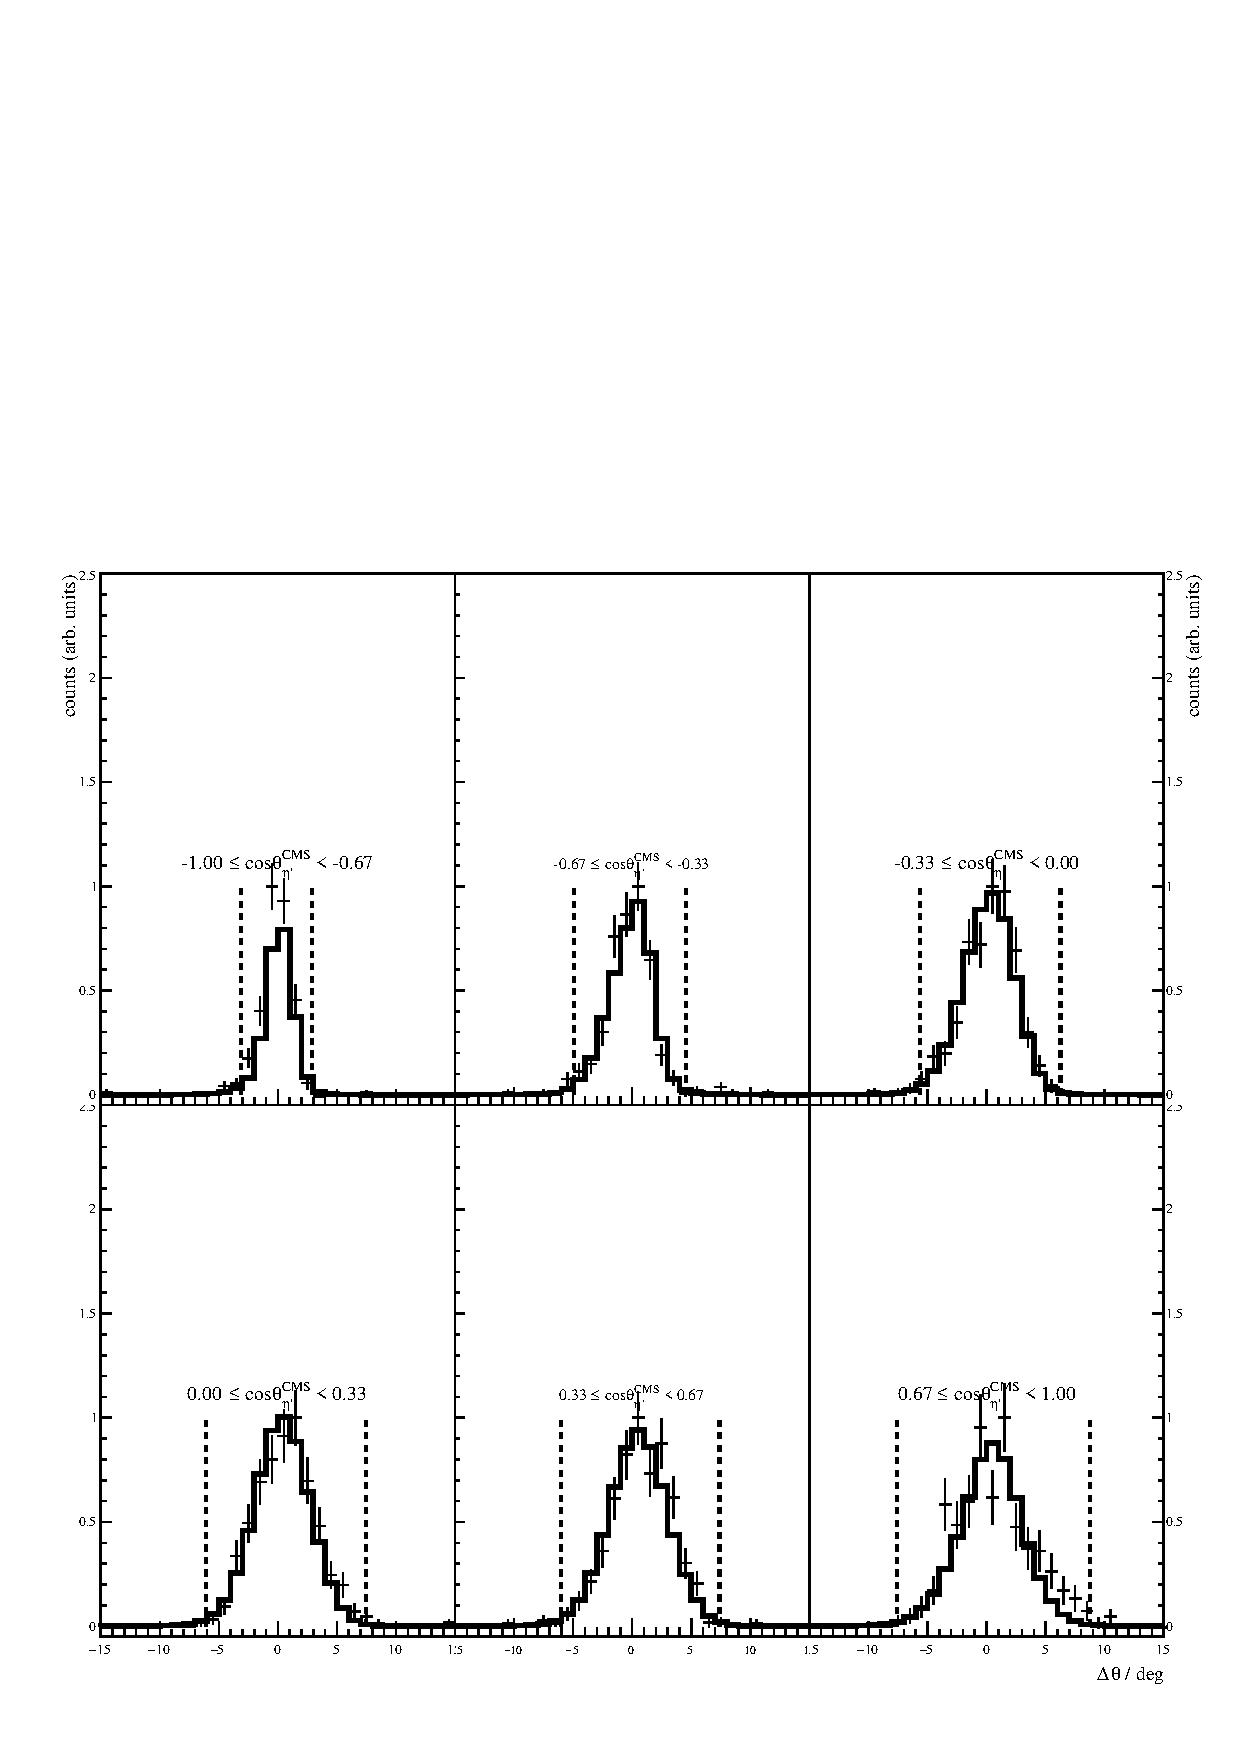
\includegraphics[width=\linewidth]{../figs/hydrogen/bin_cuts/thetacut_ebin1.pdf}
		\subcaption{$\SI{1500}{\mega\eV}\leq E_\gamma<\SI{1600}{\mega\eV}$}
	\end{subfigure}
	
	\begin{subfigure}{\linewidth}
		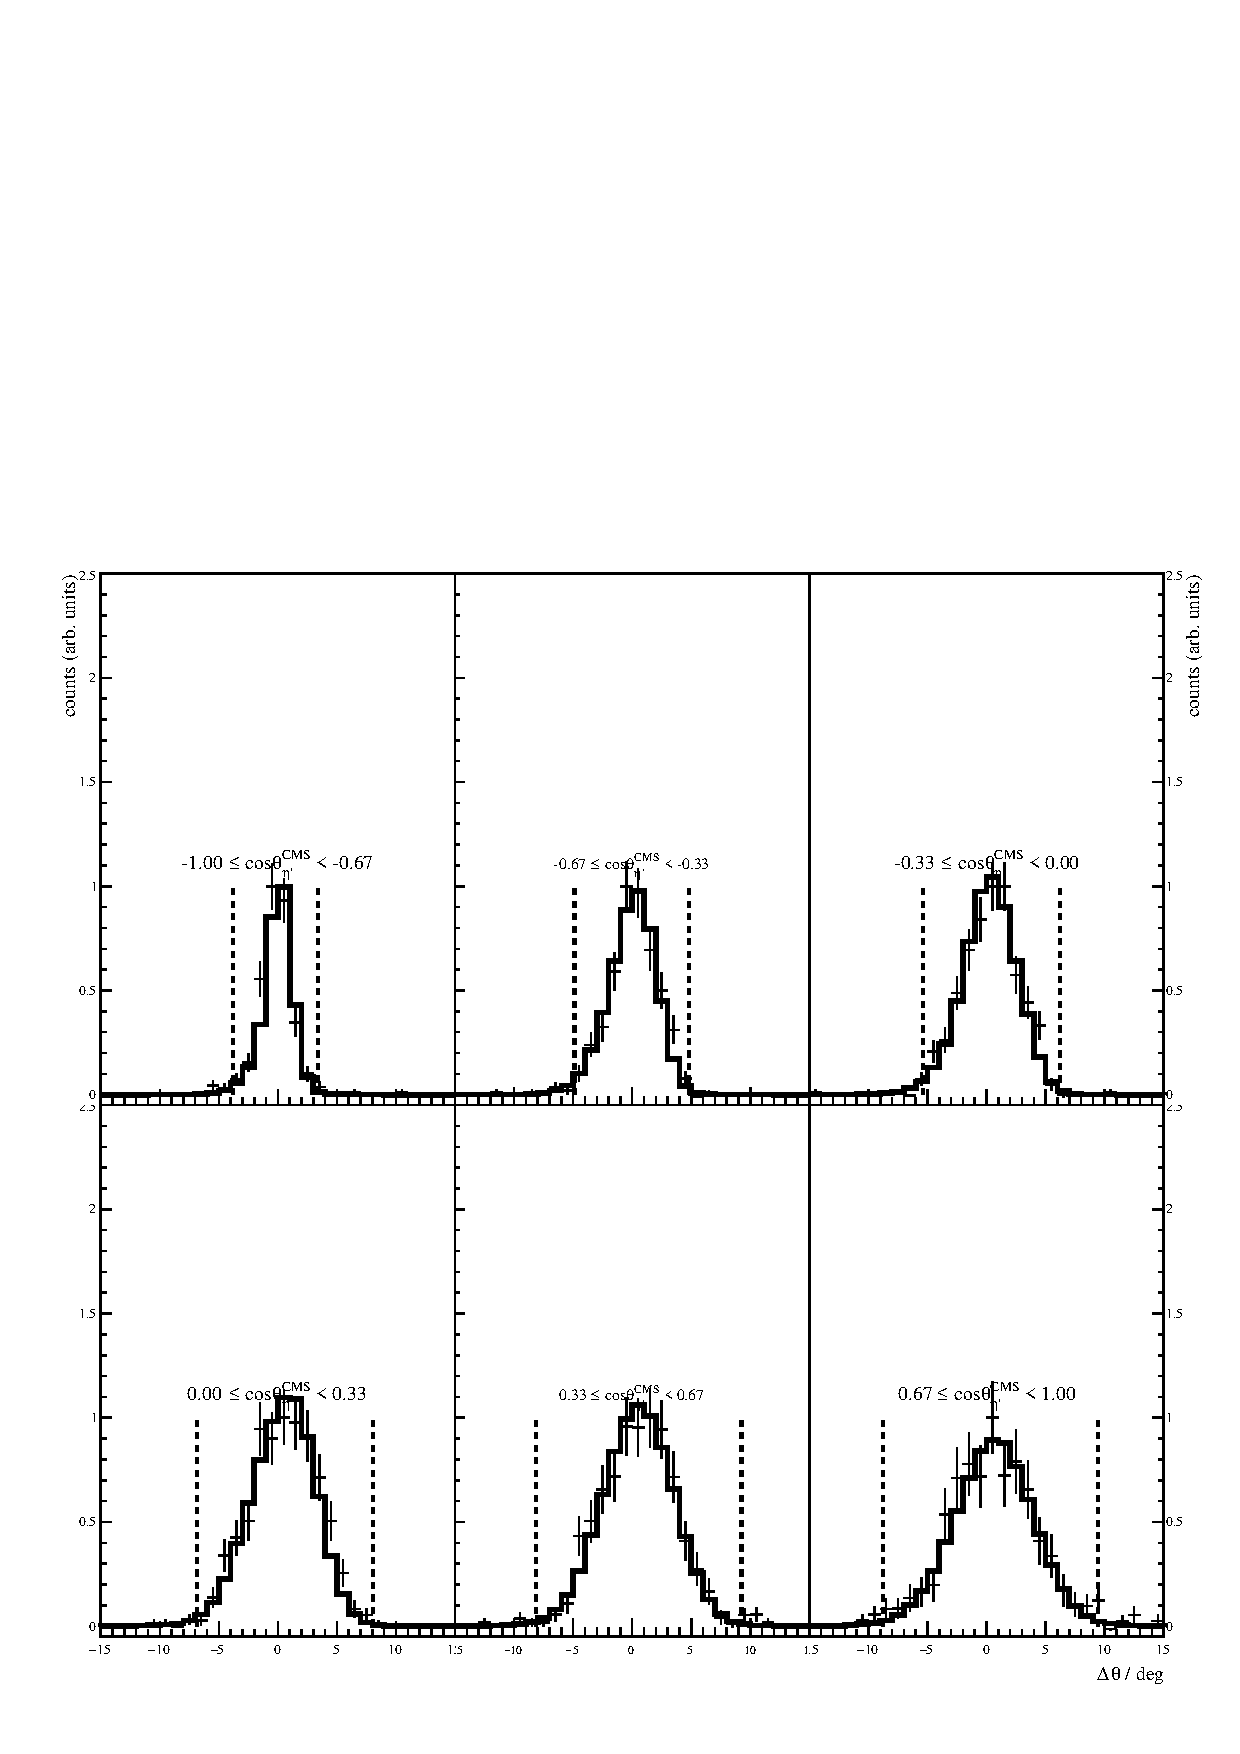
\includegraphics[width=\linewidth]{../figs/hydrogen/bin_cuts/thetacut_ebin2.pdf}
		\subcaption{$\SI{1600}{\mega\eV}\leq E_\gamma<\SI{1700}{\mega\eV}$}
	\end{subfigure}
\caption{Polar angle difference $\Delta\theta$ for all energy and angular bins. Data points are displayed as open circles, scaled Monte Carlo data belonging to $\eta'$ photoproduction is displayed as solid histogram. The determined cut ranges are indicated by the dashed red lines.}
\end{figure}
\begin{figure}[H]
	\ContinuedFloat
	\begin{subfigure}{\linewidth}
		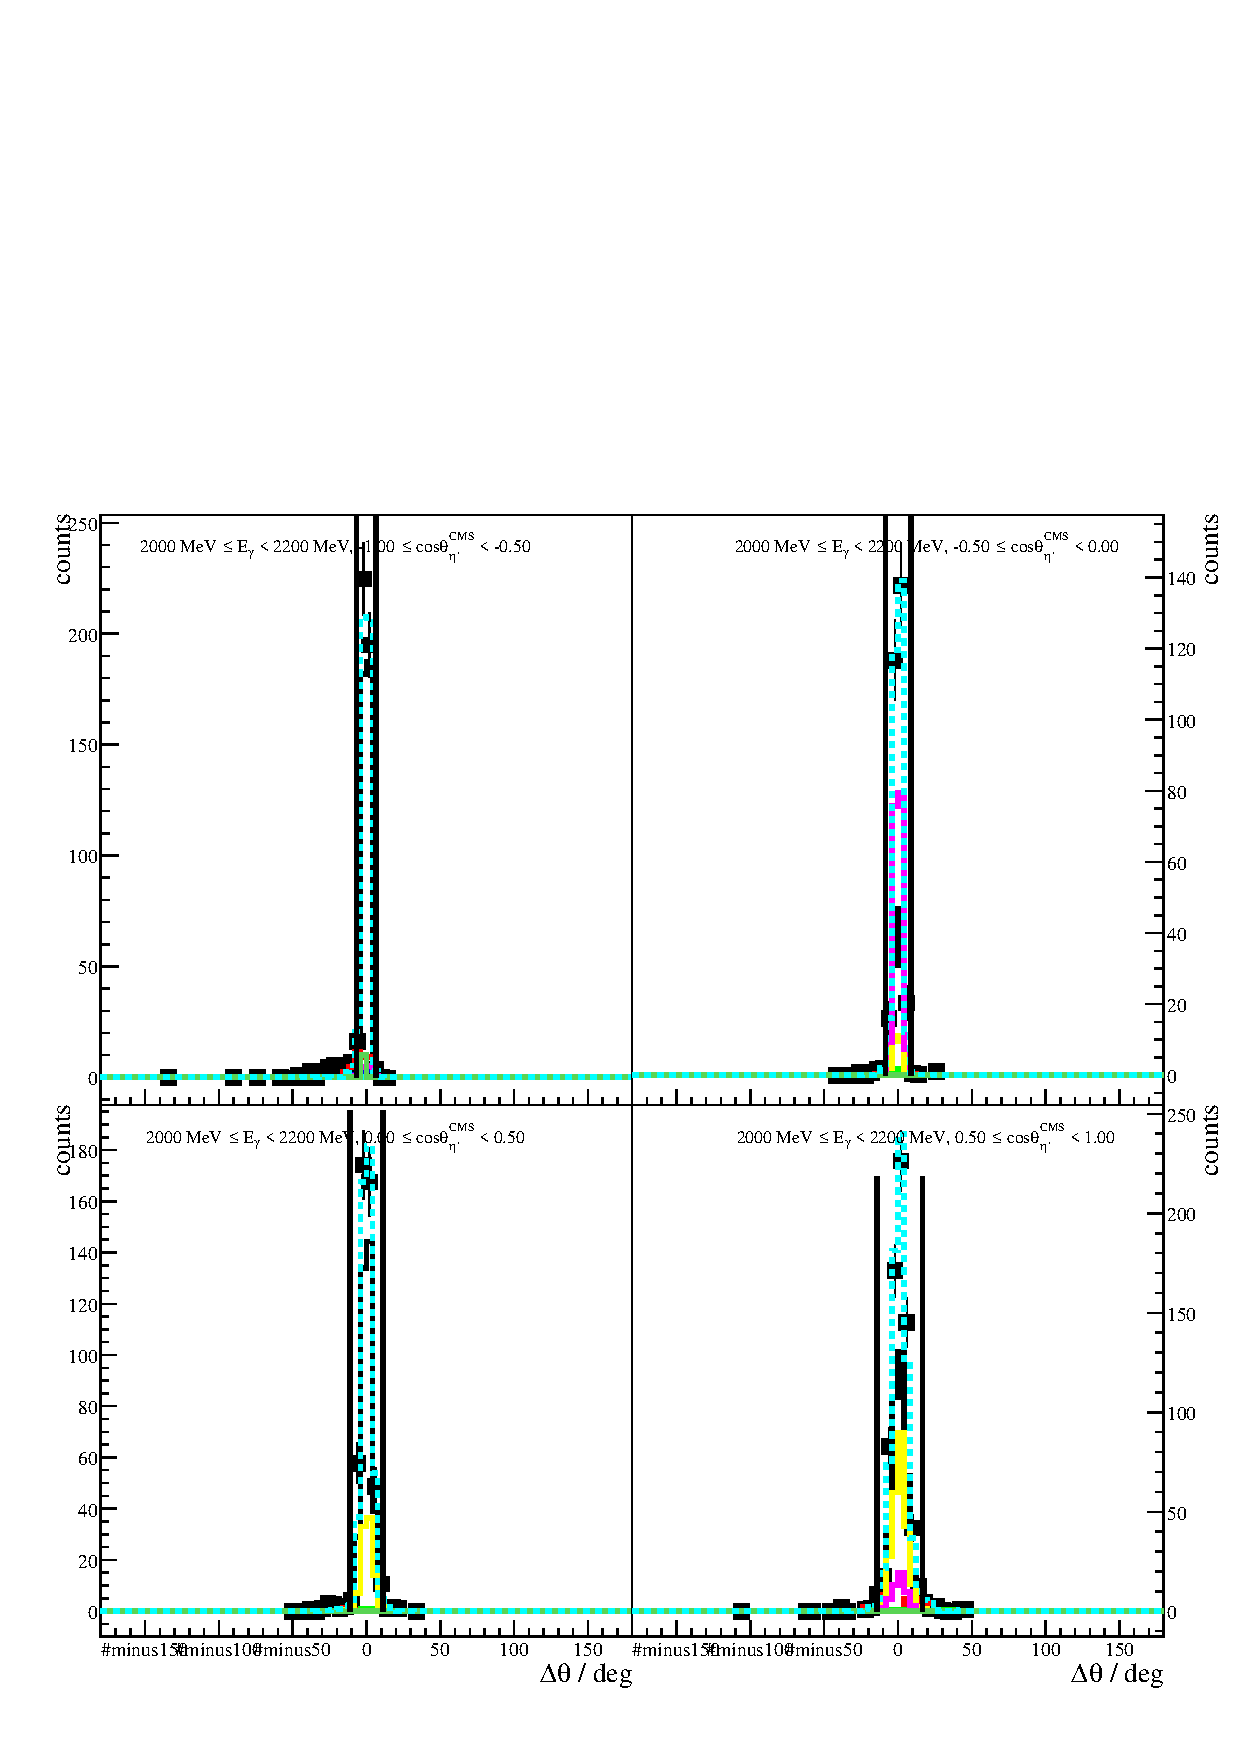
\includegraphics[width=\linewidth]{../figs/hydrogen/bin_cuts/thetacut_ebin3.pdf}
		\subcaption{$\SI{1700}{\mega\eV}\leq E_\gamma<\SI{1800}{\mega\eV}$}
	\end{subfigure}
\caption{Polar angle difference $\Delta\theta$ for all energy and angular bins. Data points are displayed as open circles, scaled Monte Carlo data belonging to $\eta'$ photoproduction is displayed as solid histogram. The determined cut ranges are indicated by the dashed red lines.}
\label{fig:apptheta}	
\end{figure}
Figure \ref{fig:apptheta} shows the polar angle difference for all energy and angular bins. Cut ranges were determined from a \textsc{Gaussian} fit to the data points. Only slight dependency on beam energy can be identified whereas clear correlation between width of the distribution and meson polar angle exists. This is due to the hit detectors which exhibit different angular resolutions, as has been discussed in the main part. Only $\eta'$ Monte Carlo data are fitted because the measured points do not give enough reference points for the fit to identify different contributing final states. There is good agreement between Monte Carlo simulations and measured data.
\newpage
\subsection{Missing mass}
\begin{figure}[H]
	\centering
	\begin{subfigure}{\linewidth}
		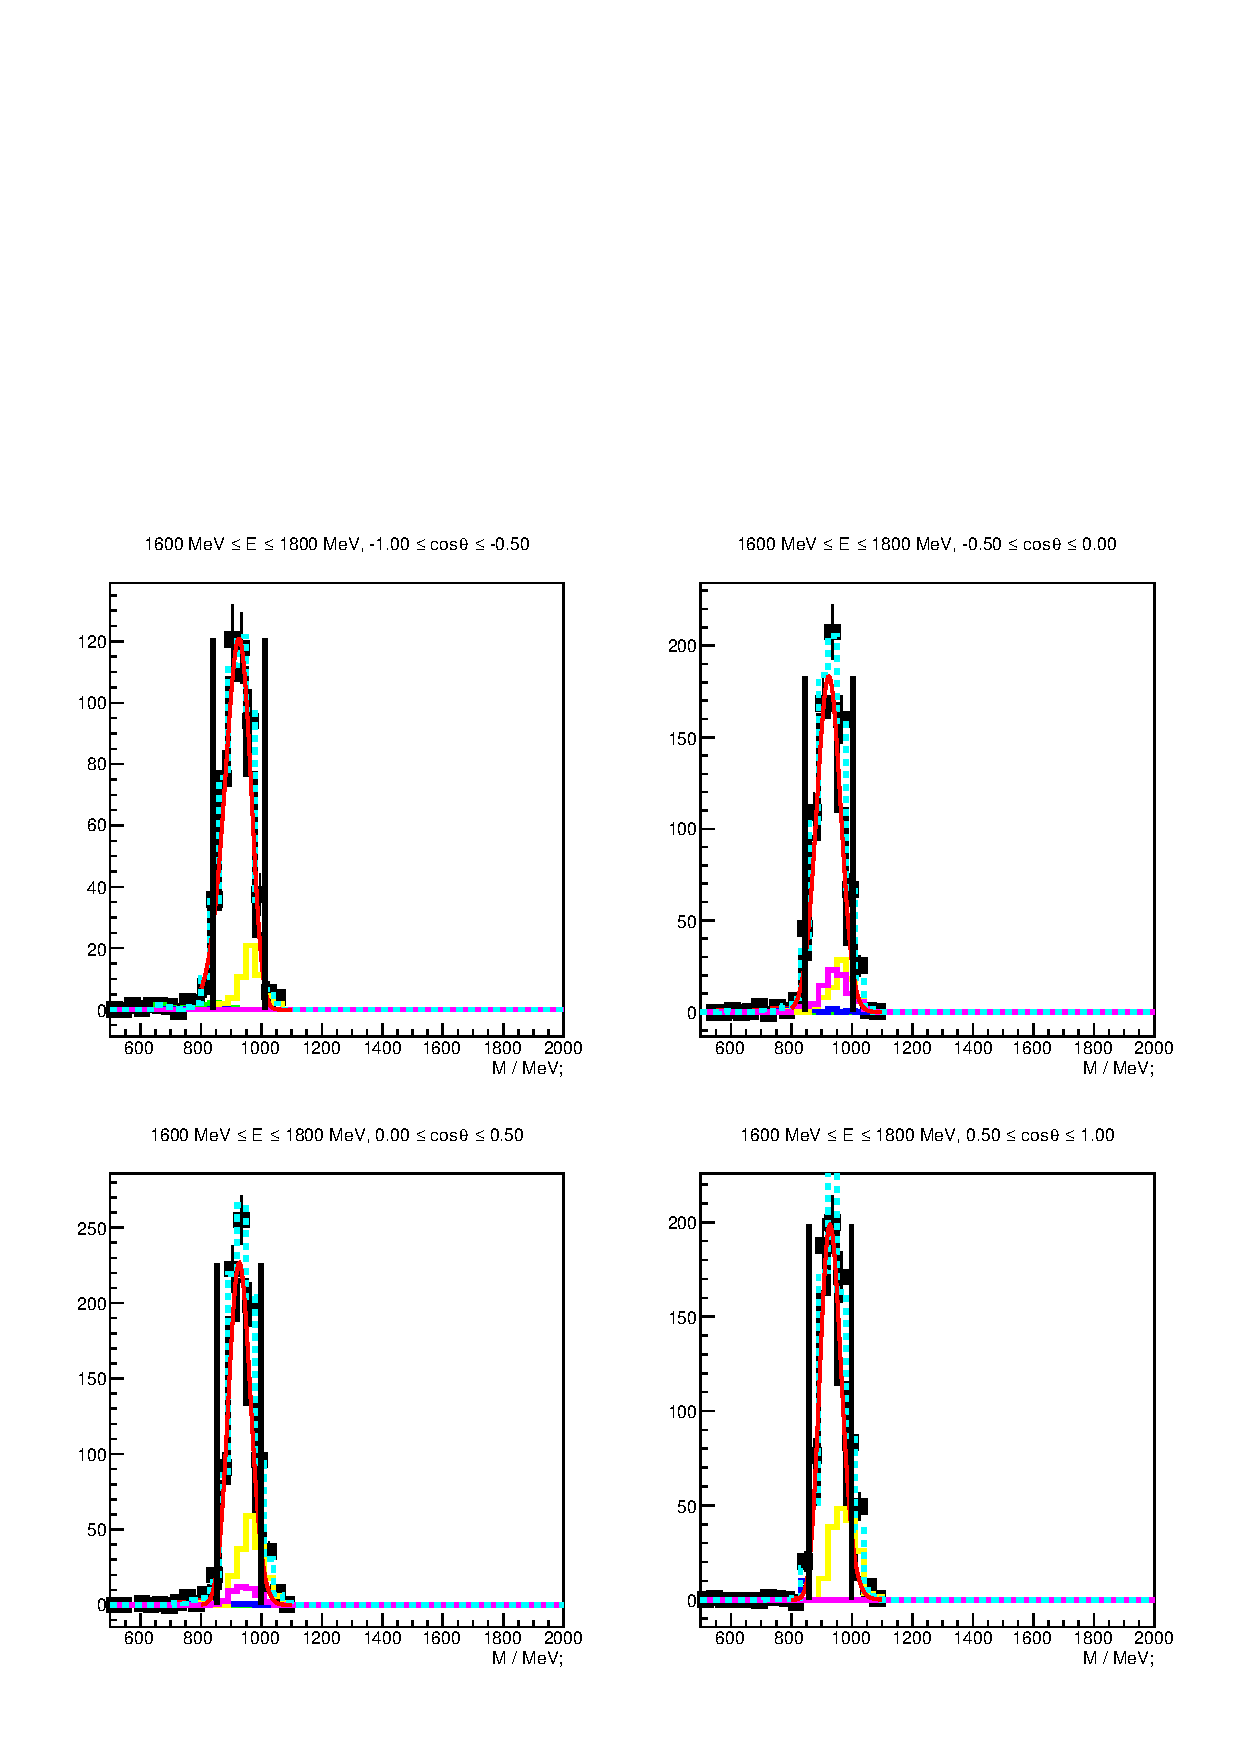
\includegraphics[width=\linewidth]{../figs/hydrogen/bin_cuts/mismcut_ebin1.pdf}
		\subcaption{$\SI{1500}{\mega\eV}\leq E_\gamma<\SI{1600}{\mega\eV}$}
	\end{subfigure}
	
	\begin{subfigure}{\linewidth}
		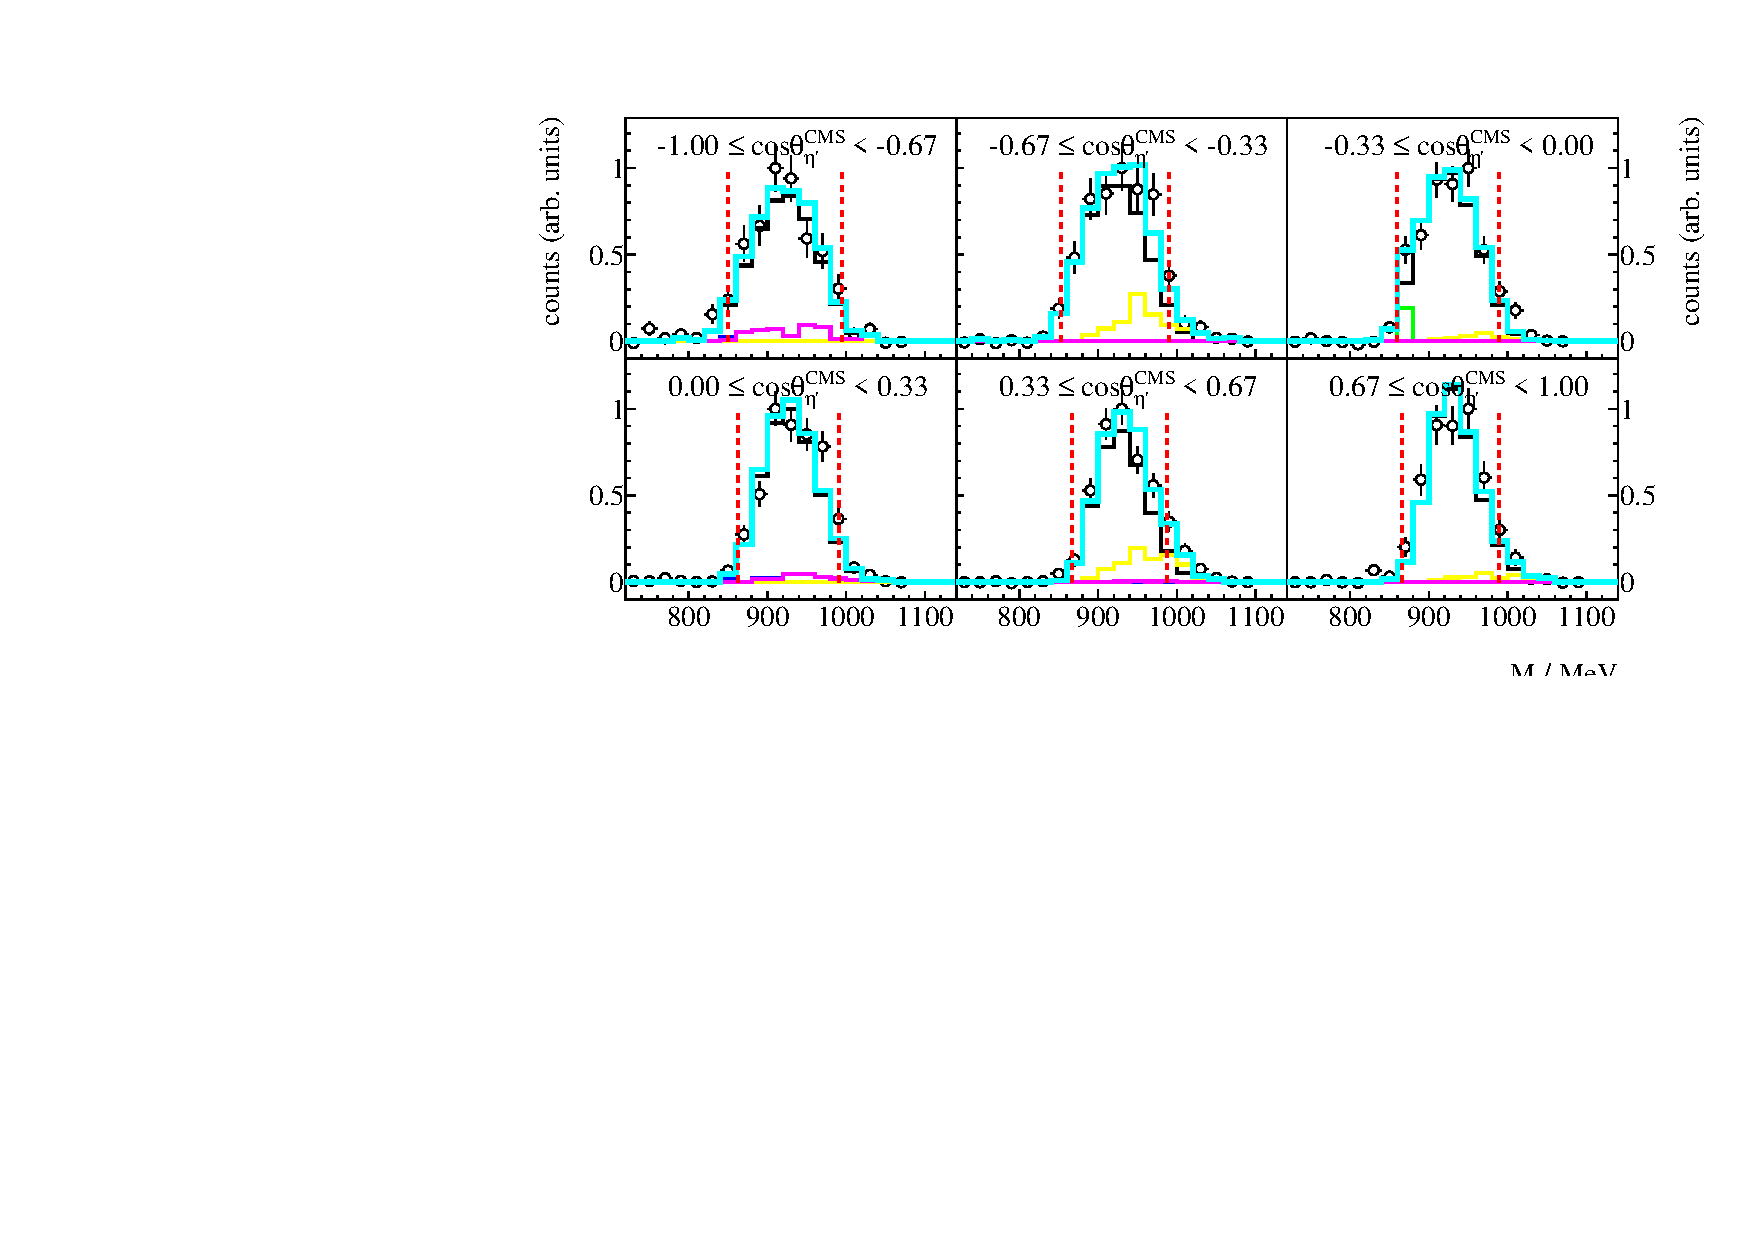
\includegraphics[width=\linewidth]{../figs/hydrogen/bin_cuts/mismcut_ebin2.pdf}
		\subcaption{$\SI{1600}{\mega\eV}\leq E_\gamma<\SI{1700}{\mega\eV}$}
	\end{subfigure}
\caption{Missing mass $m_x$ for all energy and angular bins. Data points are displayed as open circles, scaled Monte Carlo data belonging to $\eta'$ (black), $2\pi^0$ (yellow) and $\pi^0\eta$ (magenta) photoproduction is displayed as solid histogram while their sum is displayed as turquoise histogram. The determined cut ranges are indicated by the dashed red lines.}
\end{figure}
\begin{figure}[H]
	\ContinuedFloat
	\begin{subfigure}{\linewidth}
		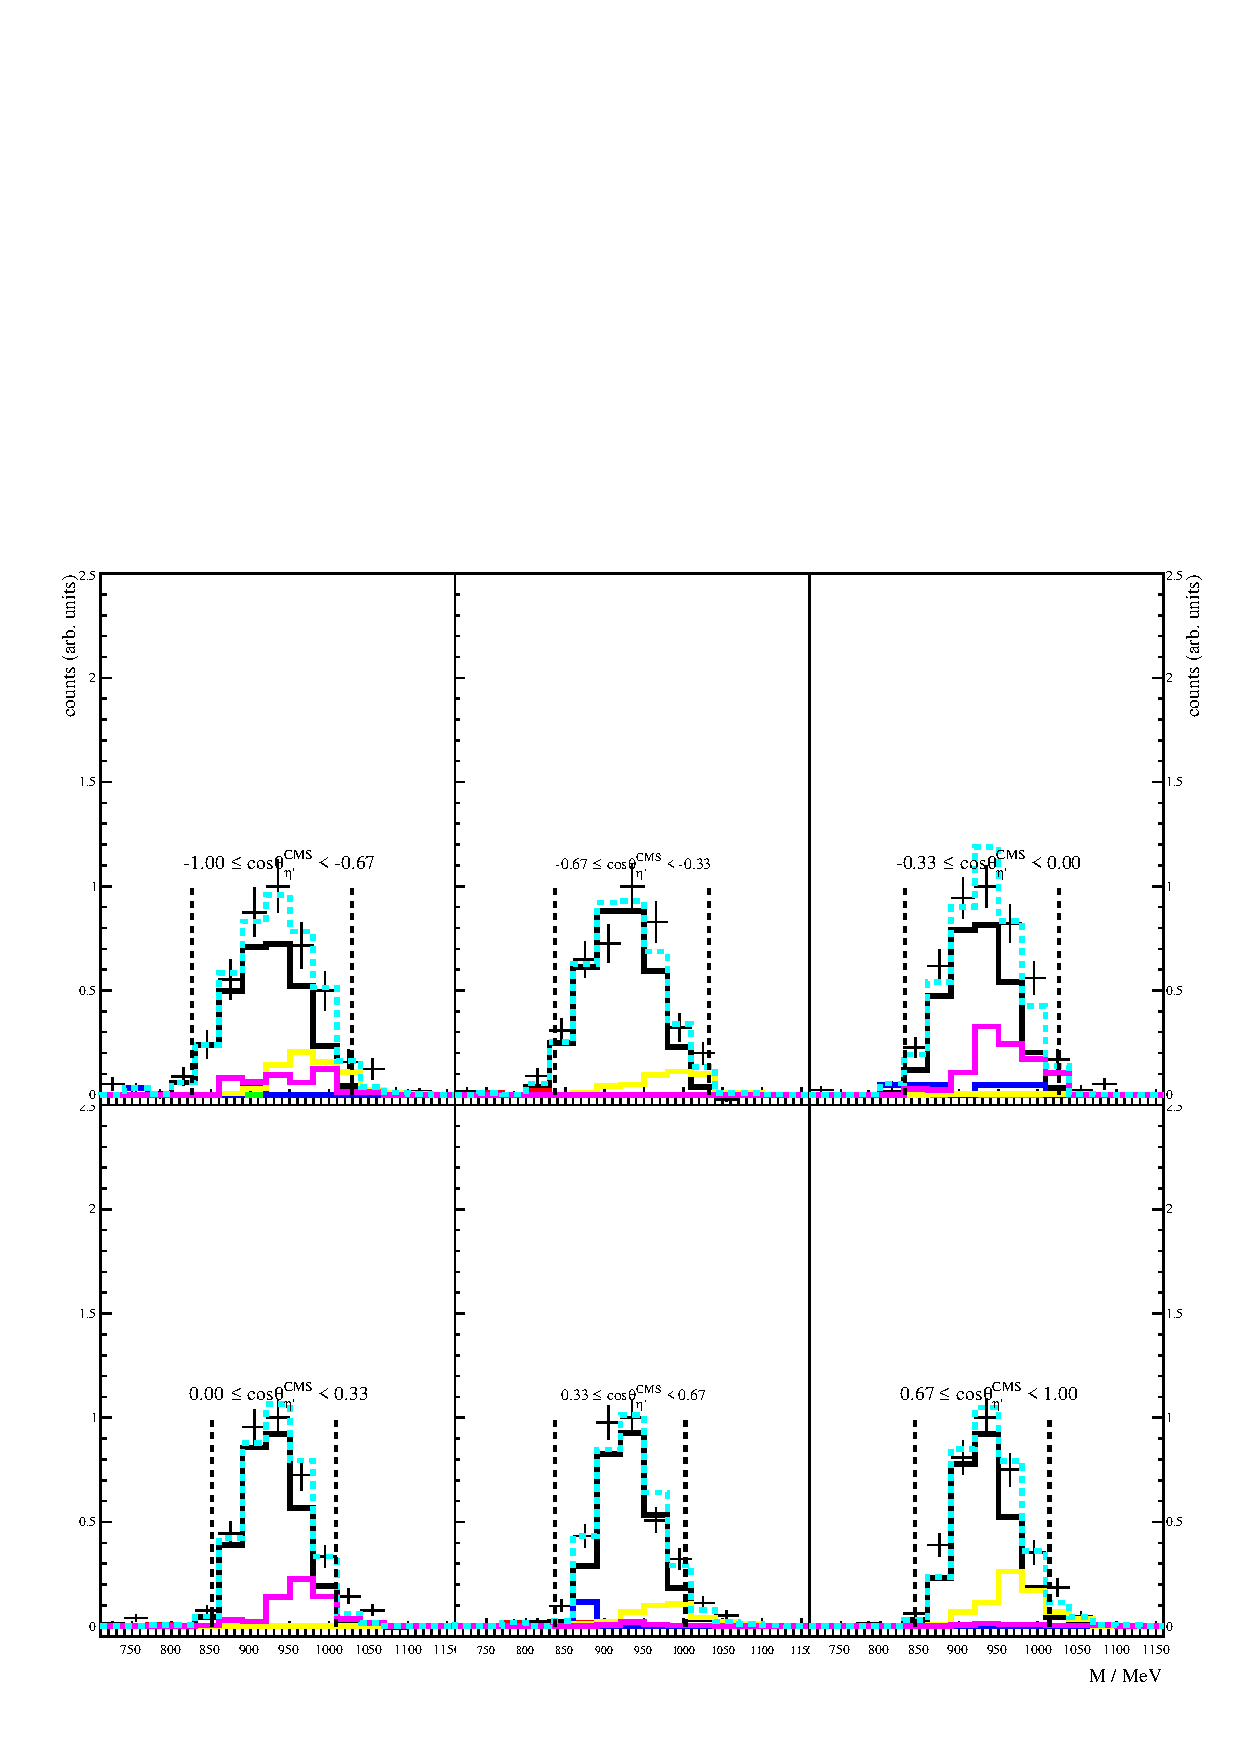
\includegraphics[width=\linewidth]{../figs/hydrogen/bin_cuts/mismcut_ebin3.pdf}
		\subcaption{$\SI{1700}{\mega\eV}\leq E_\gamma<\SI{1800}{\mega\eV}$}
	\end{subfigure}
	\caption{Missing mass $m_X$ for all energy and angular bins. Data points are displayed as open circles, scaled Monte Carlo data belonging to  $\eta'$ (black), $2\pi^0$ (yellow) and $\pi^0\eta$ (magenta) photoproduction is displayed as solid histogram while their sum is displayed as turquoise histogram. The determined cut ranges are indicated by the dashed red lines.}
	\label{fig:appmism}
\end{figure}
Figure \ref{fig:appmism} shows the missing mass for all energy and angular bins. Cut ranges were determined from a \textsc{Novosibirsk} fit to the Monte Carlo data. Only slight dependency on meson polar angle can be identified. Especially at higher beam energies the missing mass peak grows wider with flat background contributions from $2\pi^0$ and $\pi^0\eta$ production towards higher masses. The Monte Carlo fit mostly shows consistency with the fit of the invariant mass spectra. However, spectra are to be seen with caution, since the shapes of the two different background contributions are very similar and there is no other reference point in the missing mass spectrum as opposed to the invariant mass. Fits to the invariant mass spectra may reveal background contributions where a fit to the missing mass spectrum failed to find any. There is good agreement between Monte Carlo simulations and measured data.
\newpage
\subsection{Invariant mass}
\begin{figure}[H]
	\centering
	\begin{subfigure}{\linewidth}
		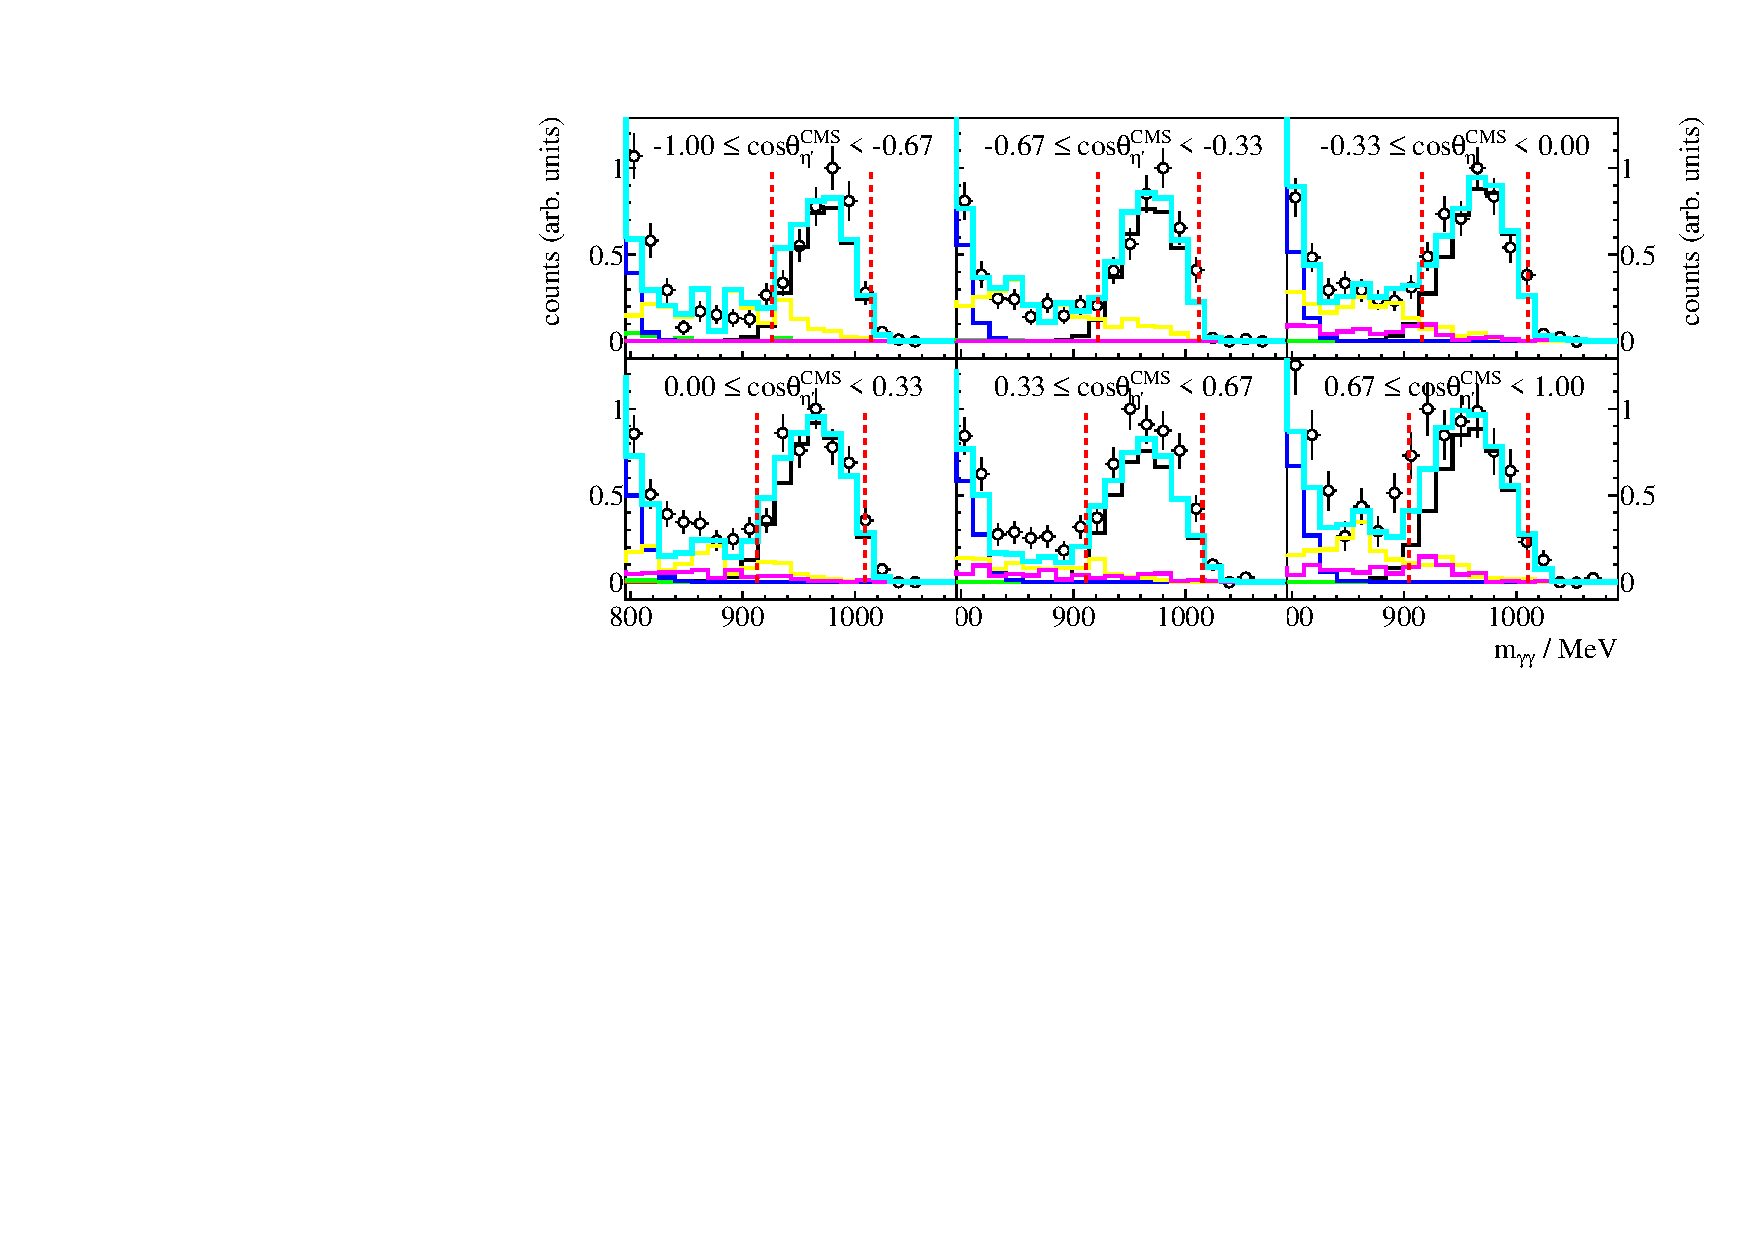
\includegraphics[width=\linewidth]{../figs/hydrogen/bin_cuts/invcut_ebin1.pdf}
		\subcaption{$\SI{1500}{\mega\eV}\leq E_\gamma<\SI{1600}{\mega\eV}$}
	\end{subfigure}
	
	\begin{subfigure}{\linewidth}
		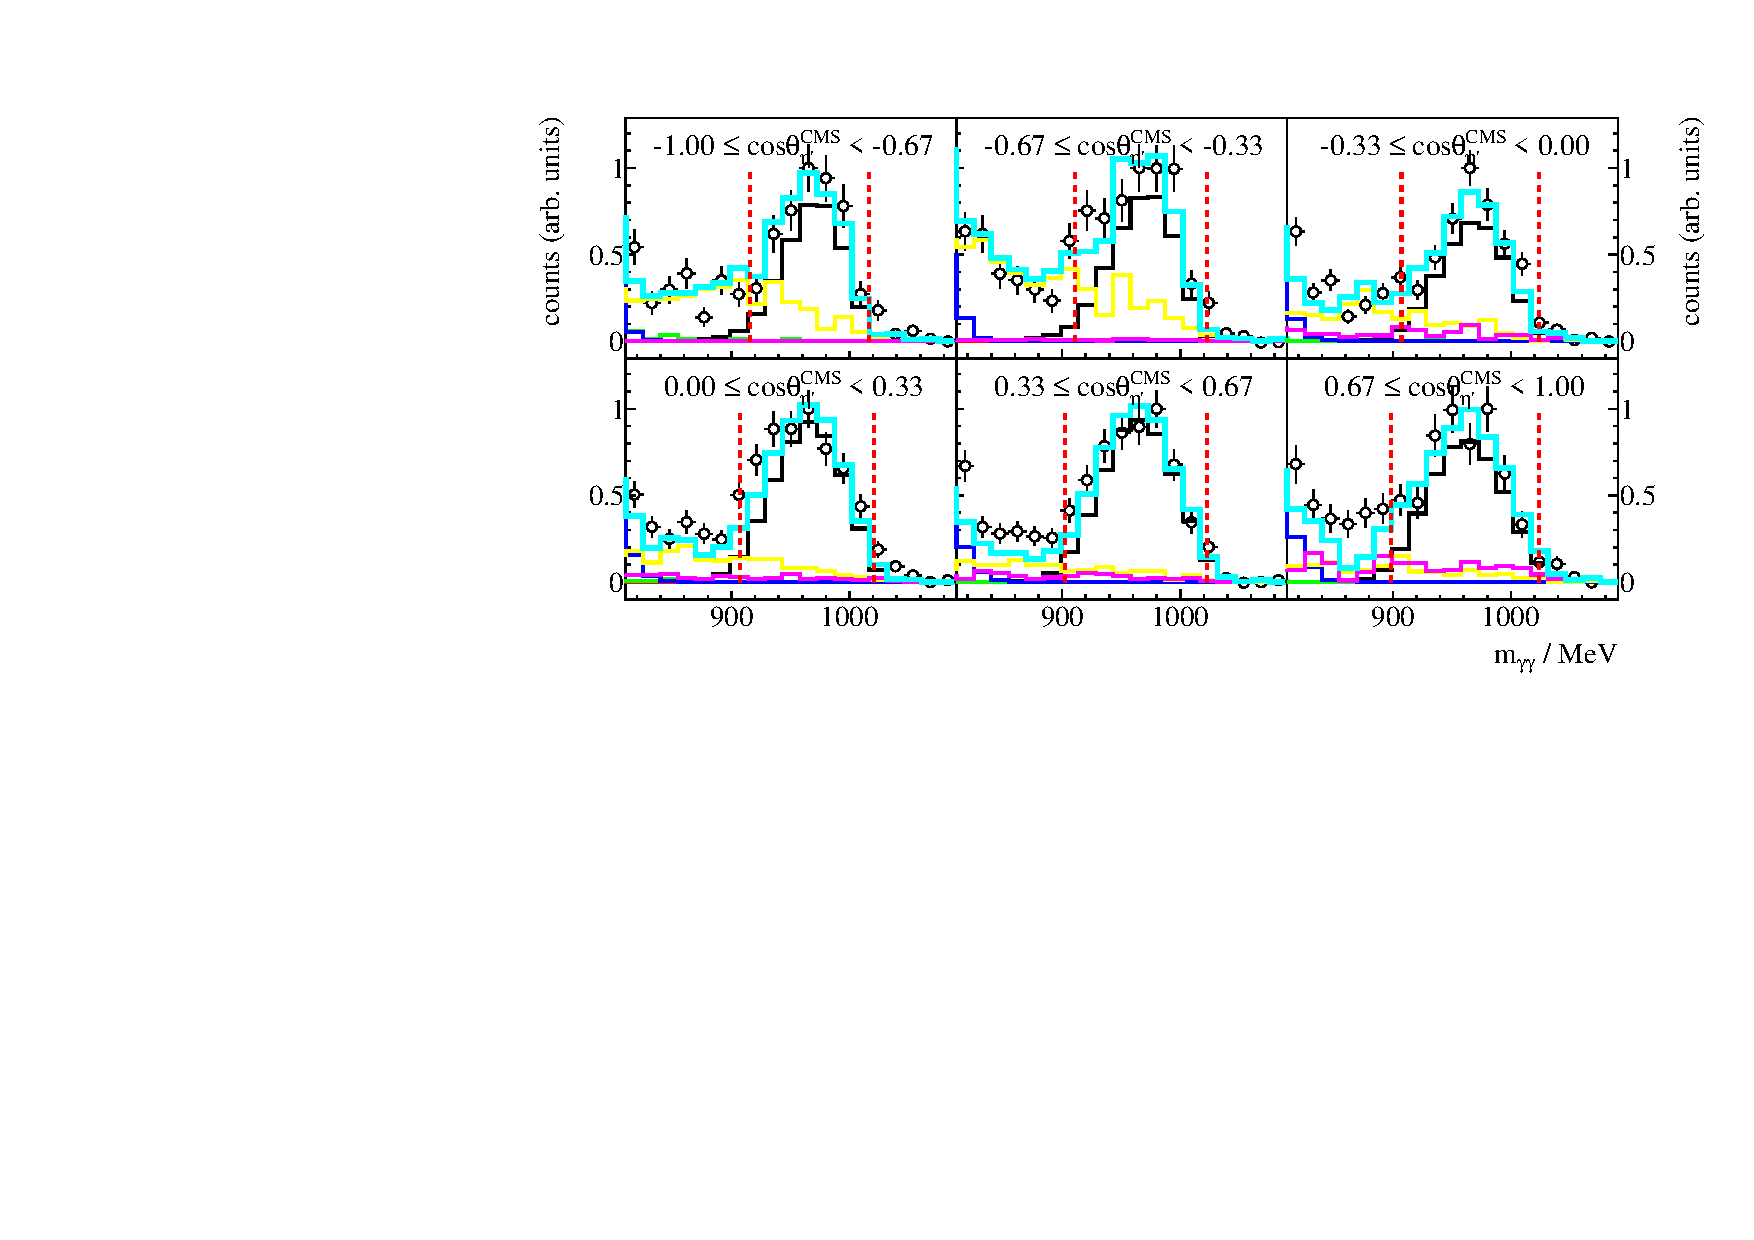
\includegraphics[width=\linewidth]{../figs/hydrogen/bin_cuts/invcut_ebin2.pdf}
		\subcaption{$\SI{1600}{\mega\eV}\leq E_\gamma<\SI{1700}{\mega\eV}$}
	\end{subfigure}
\caption{Invariant mass $m_\text{meson}$ for all energy and angular bins. Data points are displayed as open circles, scaled Monte Carlo data belonging to $\eta'$ (black), $2\pi^0$ (yellow), $\pi^0\eta$ (magenta), $\pi^0$ (green) and $\omega$ (blue) photoproduction is displayed as solid histogram while their sum is displayed as turquoise histogram. The determined cut ranges are indicated by the dashed red lines.}
\end{figure}
\begin{figure}[H]
	\ContinuedFloat
	\begin{subfigure}{\linewidth}
		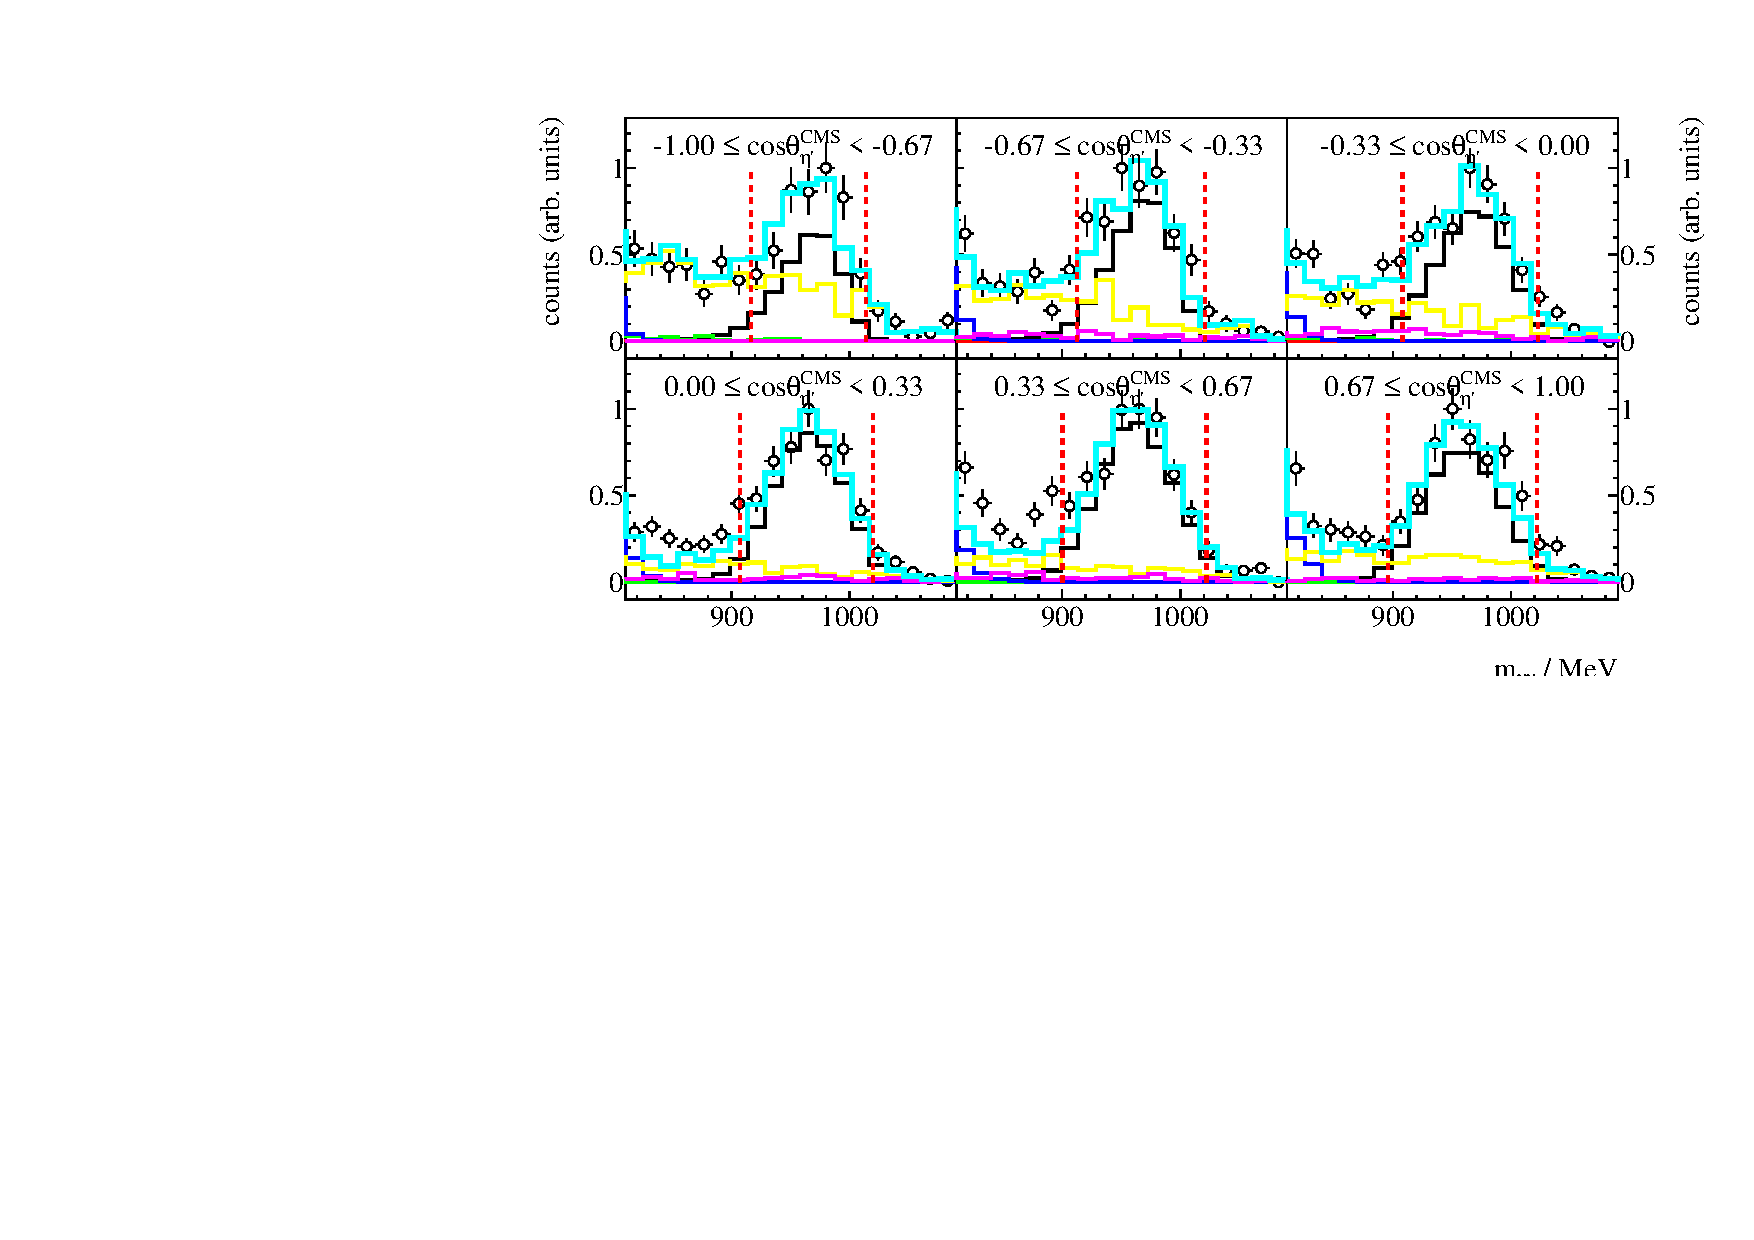
\includegraphics[width=\linewidth]{../figs/hydrogen/bin_cuts/invcut_ebin3.pdf}
		\subcaption{$\SI{1700}{\mega\eV}\leq E_\gamma<\SI{1800}{\mega\eV}$}
	\end{subfigure}
\caption{Invariant mass $m_\text{meson}$ for all energy and angular bins. Data points are displayed as open circles, scaled Monte Carlo data belonging to $\eta'$ (black), $2\pi^0$ (yellow), $\pi^0\eta$ (magenta), $\pi^0$ (green) and $\omega$ (blue) photoproduction is displayed as solid histogram while their sum is displayed as turquoise histogram. The determined cut ranges are indicated by the dashed red lines.}
\label{fig:appinv}
\end{figure}
Figure \ref{fig:appinv} shows the invariant mass for all kinematic bins. Hardly any dependence on meson direction and beam energy is observed. However, background contributions are especially observed in very forward and backward direction towards higher beam energies in consistency with findings from the missing mass spectra.  A flat background is realized by $2\pi^0$ and $\pi^0\eta$ production. There is good agreement between Monte Carlo simulations and measured data.
\chapter{Discussion of binned fits}
\label{app:binnedfits}
Investigation of toy Monte Carlo experiments (cf. section \ref{sec:sigma_etap}) revealed that the choice of binning leads to systematic errors regarding the parameter $\Sigma$ when fitting a binned distribution to the equation 
\begin{equation}
	A\left(\phi\right)=\Sigma\cdot\cos\left(2\left(\alpha^\parallel-\phi\right)\right).
\end{equation}
To investigate this further, the distributions $A\left(\phi\right)$ from different toy Monte Carlo experiments where fitted for several binnings in $\phi$. Three different Monte Carlo experiments were considered, each corresponding roughly to the expected statistics in one kinematic bin for $\pi^0$, $\eta$ and $\eta'$ photoproduction, respectively. For simplicity's sake, only least squares fits are shown here, although similar results were found for \textsc{Bayesian} fits also. The equivalency of \textsc{Bayesian} and least squares fit has been demonstrated sufficiently up until now. To identify the bias that is introduced by binning the data, 10000 toy Monte Carlo bins for each setting are fitted for $n=10,15,20,\dots,100$ bins. Then the dependence from the amount of bins of the mean $\mu$ of the normalized residuals $\xi$ as well as the mean $\chi^2$ value of all fits is investigated. This is shown in Figure \ref{fig:appbin}; The fitted mean of the normalized posteriors $\xi$ is plotted against the number of bins (blue data points, left ordinate) as well as the mean $\chi^2$ of 10000 fits depending on the number of bins (red data points, right ordinate). Clear dependencies can be made out: while too few bins tend to underestimate the true value of the beam asymmetry, too much bins will lead to an overcompensation. For this reason, the functions $\chi^2(n)$ and $\mu(n)$ are monotonously rising with increasing number of bins $n$. An exception is realized by the samples that simulated the statistics of the $\eta'$ final state, which can be explained by the fact, that after reaching a certain number of bins, no sensible fit estimates can be made anymore because too few data points are available. A minimum deviation from the nominal value is reached with $n=10,20,30$ bins for statistics comparable to $\eta',\eta$ and $\pi^0$ production respectively. This does not coincide with a minimum $\chi^2$ necessarily, although the mean $\chi^2$ values associated with the best estimation of the input value are compatible with 1. Figure \ref{fig:appbin} however remarkably shows the influence binning has on the extraction of the beam asymmetry. Since there exist other methods, binned fits should only be used as a sanity check, but generally avoided, to circumvent the introduction of any systematics inherent to binning.
\begin{figure}[htbp]
	\centering
	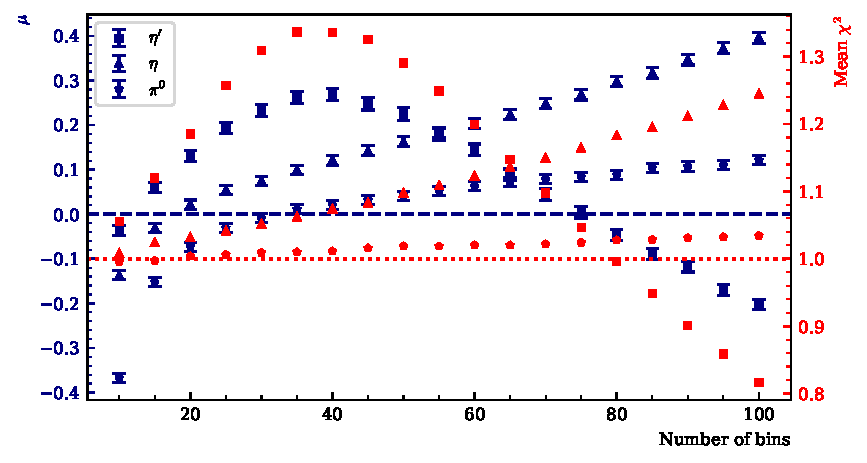
\includegraphics[width=\linewidth]{../bayes/toyMC/plots/binnedfits.pdf}
	\caption{Fit performance in dependence of the number of bins. Left axis shows the mean $\mu$ of the distribution of the normalized residuals $\xi$, right axis shows the mean $\chi^2$ of all fits. Squares simulate fits with statistics similar to the $\gamma p \to p\eta'\to p\gamma\gamma$ final state, triangles statistics similar to the $\gamma p\to p\eta\to p\gamma\gamma$ and final state, pentagons statistics similar to the $\gamma p \to p \pi^0\to p\gamma\gamma$. Dotted red line indicates the ideal value of $\chi^2=1$, while the dashed blue line indicates the ideal mean of the normalized residuals at $\mu=0$.}
	\label{fig:appbin}
\end{figure}
\chapter{Investigation of posteriors without truncation}
\label{app:trunc}
In section \ref{sec:sigma_etap} the investigation of posterior distributions from unbinned \textsc{Bayesian} fits was incomplete, since the normalized residuals as well as the likelihood pool could not be built with truncated posteriors. This is now supplemented here. After the fits have been repeated without implementing a truncation for the posteriors, all introduced measures to argue good fit quality can be examined. As a reminder, the data were generated with $\Sigma_1=0.5$ and $\Sigma_t=-0.5$. Figure \ref{fig:completpost} shows the combined posteriors of all fits. The left hand side shows the normalized residuals $\Xi$ and the right hand side the unnormalized combination of all posteriors. The results completely meet the expectations, the input values for the beam asymmetries are very well reproduced, and the normalized residuals follow a standard normal distribution as \textsc{Gaussian} fits show. Together with the results obtained from the independent likelihood pool (Figure \ref{fig:applik}), which is able to reproduce the input values within $1\sigma$, this suffices to conclude correct estimation of distribution widths with no inherent bias, as had already been found in section \ref{sec:sigma_eta}.

\begin{figure}[htbp]
	\begin{subfigure}{\linewidth}
		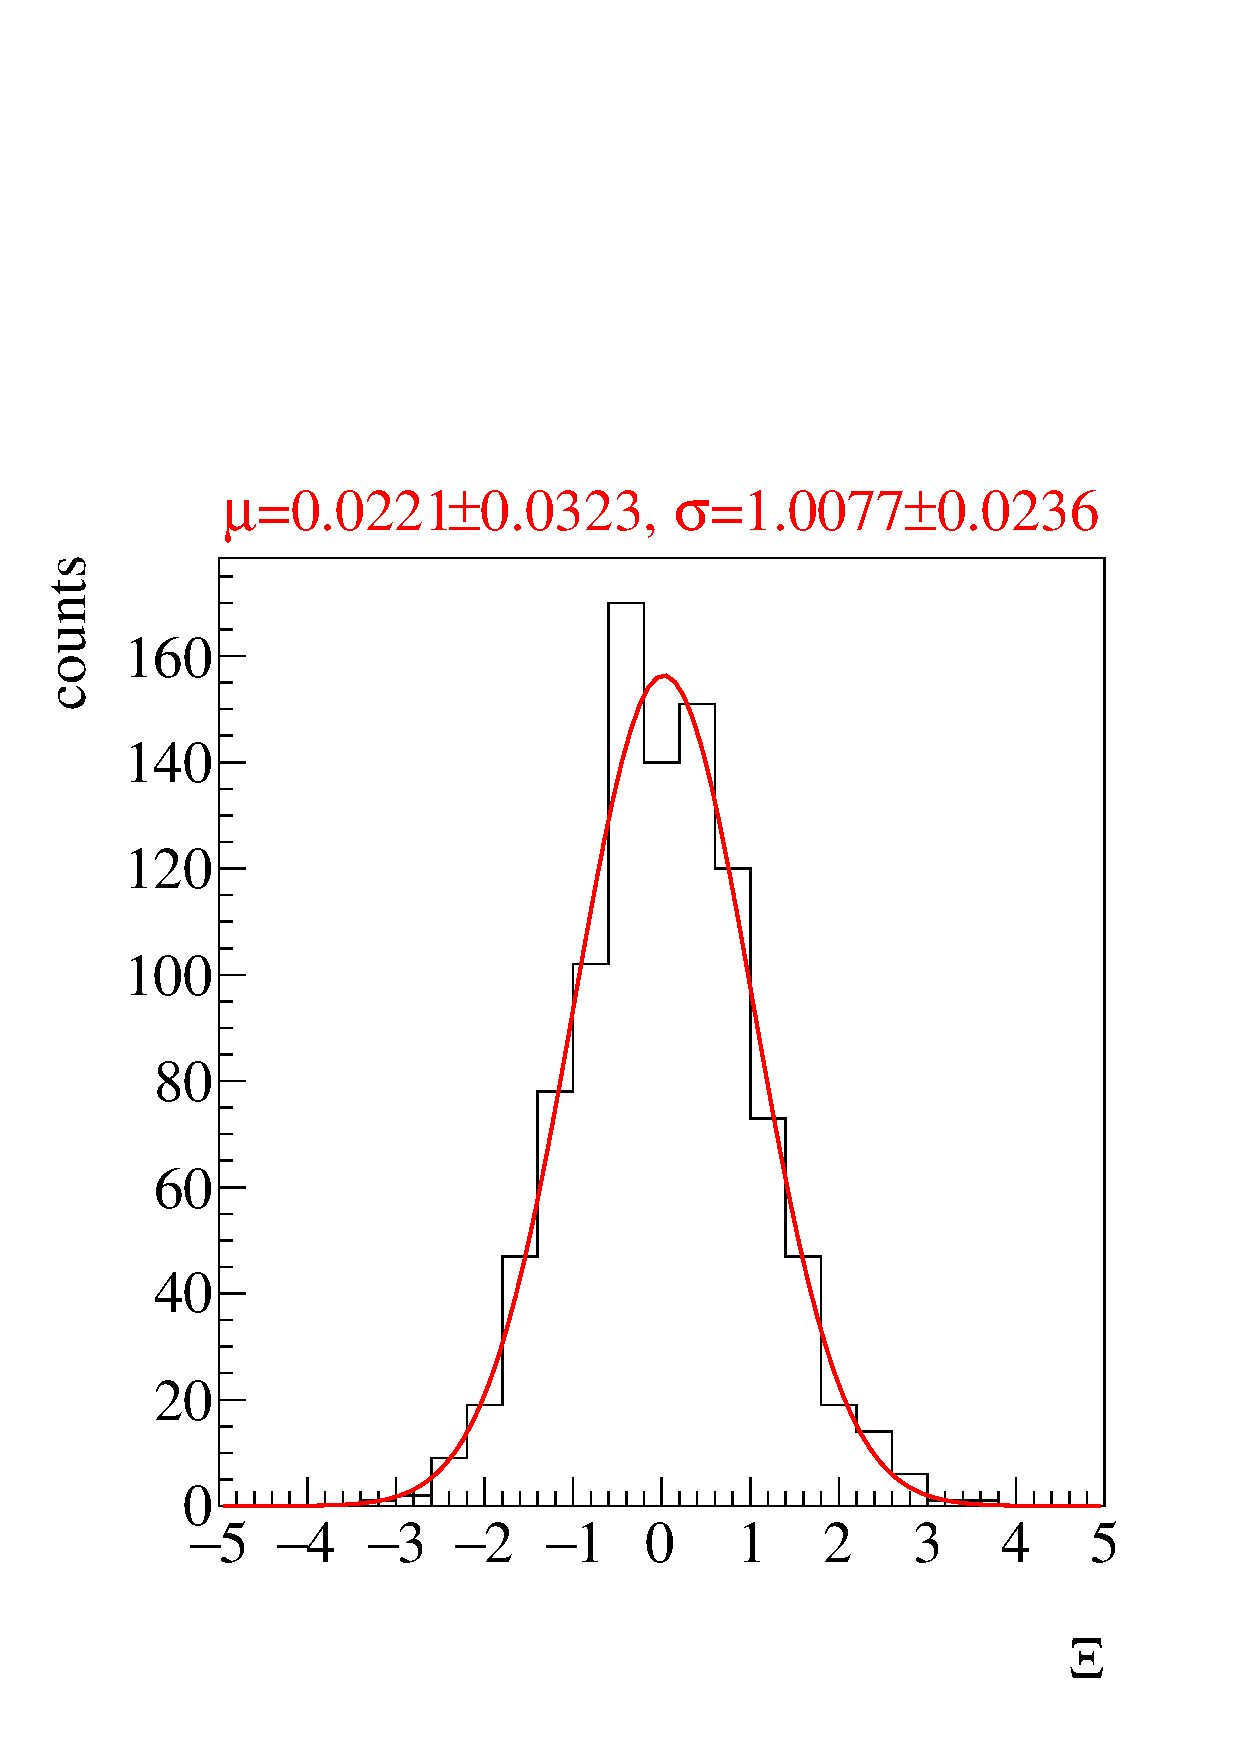
\includegraphics[width=.49\linewidth]{../bayes/etap_event_based_fit/plots/combined_post_add_notrunc.pdf}
		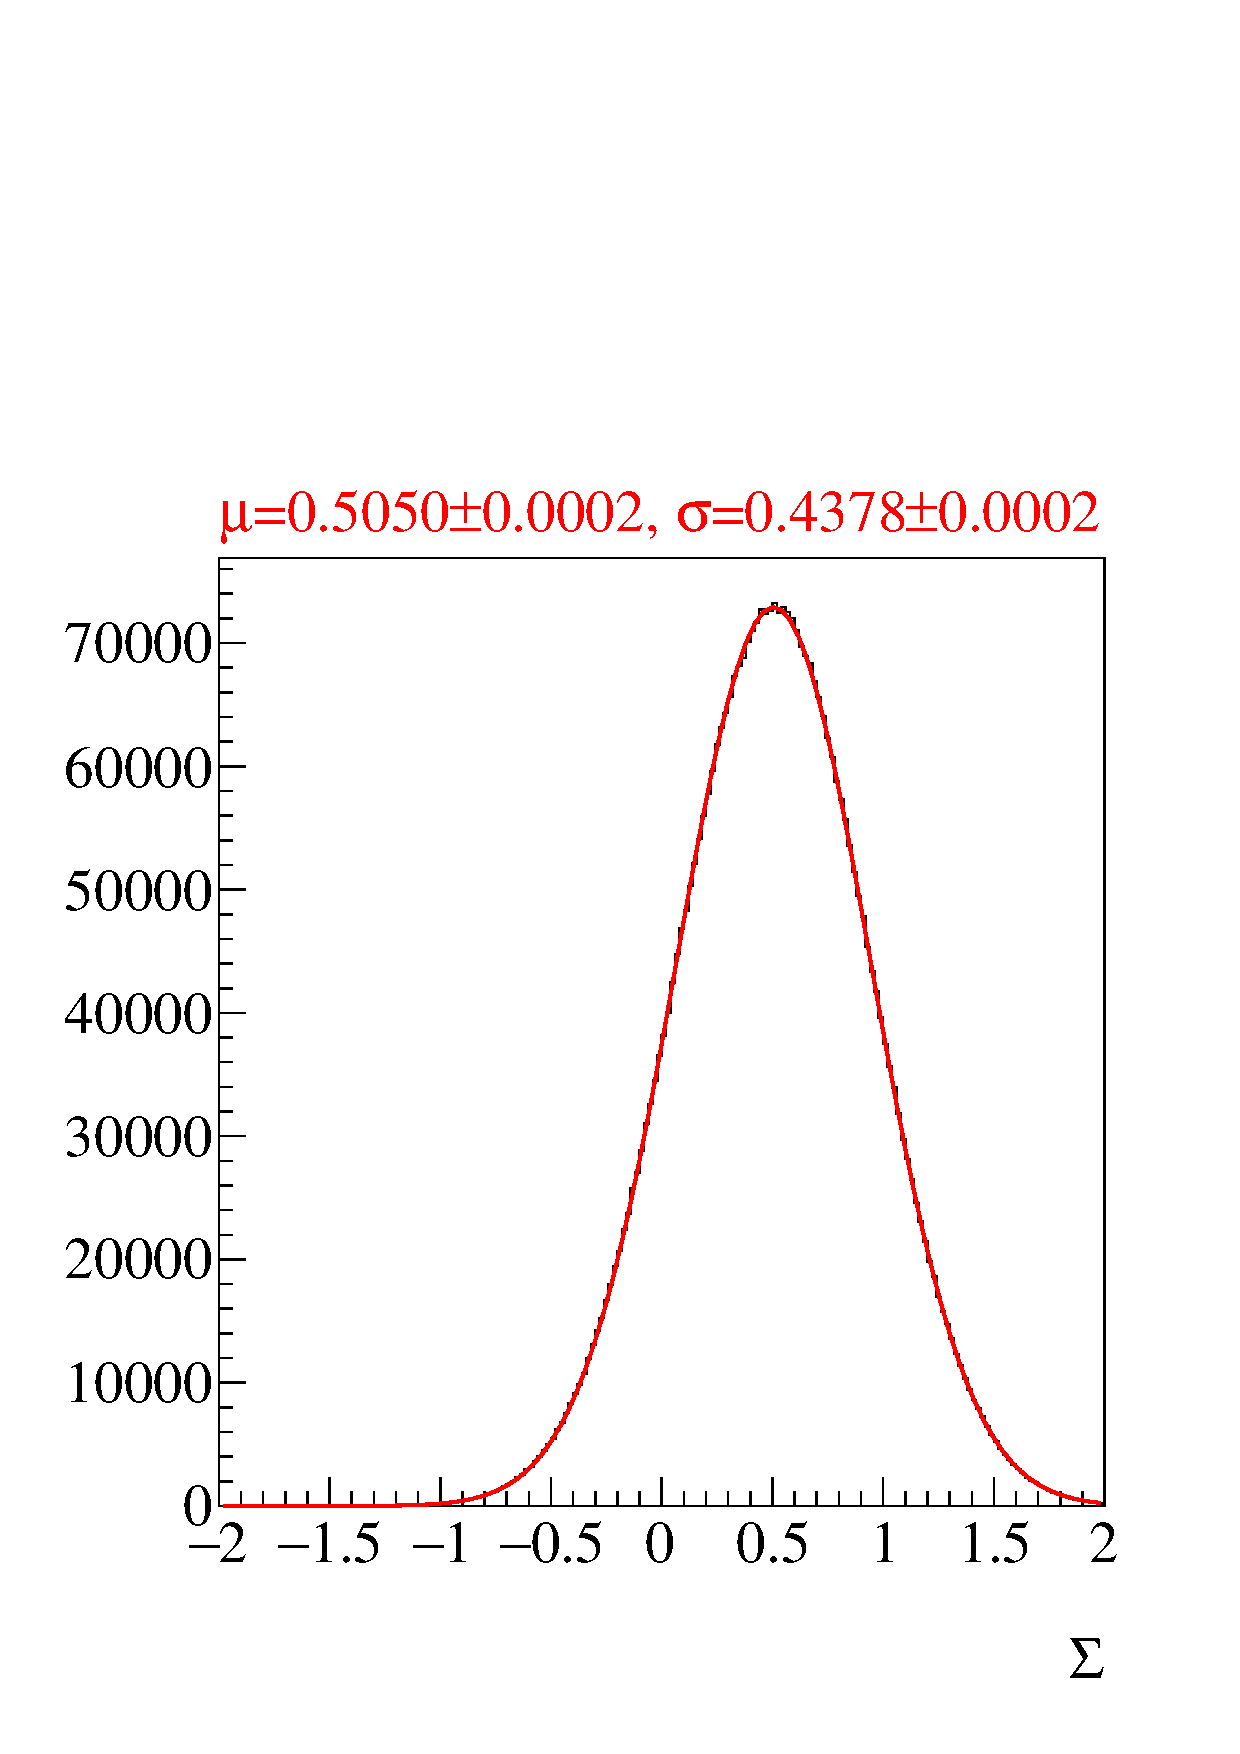
\includegraphics[width=.49\linewidth]{../bayes/etap_event_based_fit/plots/combined_post_add_notrunc_raw.pdf}
		\subcaption{Beam asymmetry $\Sigma_1$}
	\end{subfigure}
	\begin{subfigure}{\linewidth}
	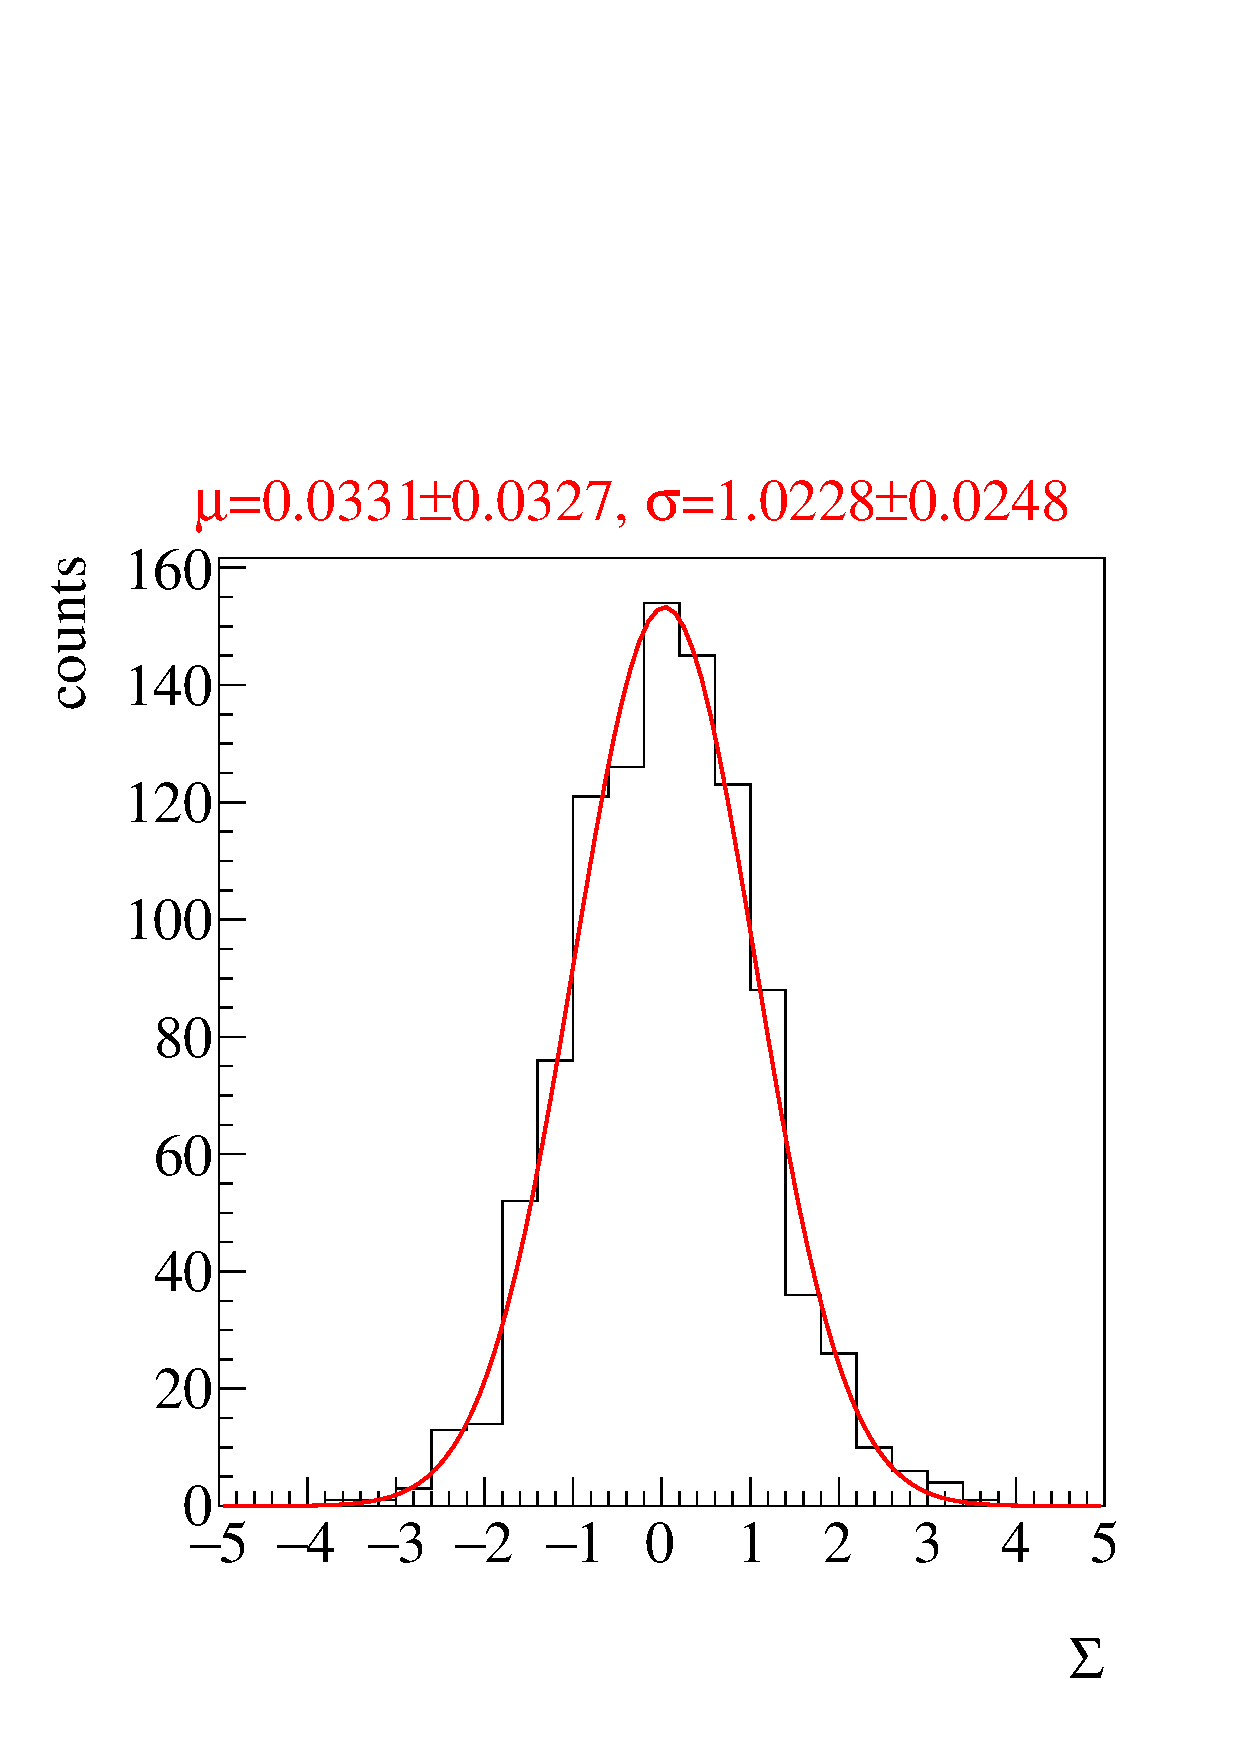
\includegraphics[width=.49\linewidth]{../bayes/etap_event_based_fit/plots/combined_post_add_notrunc_bkg.pdf}
	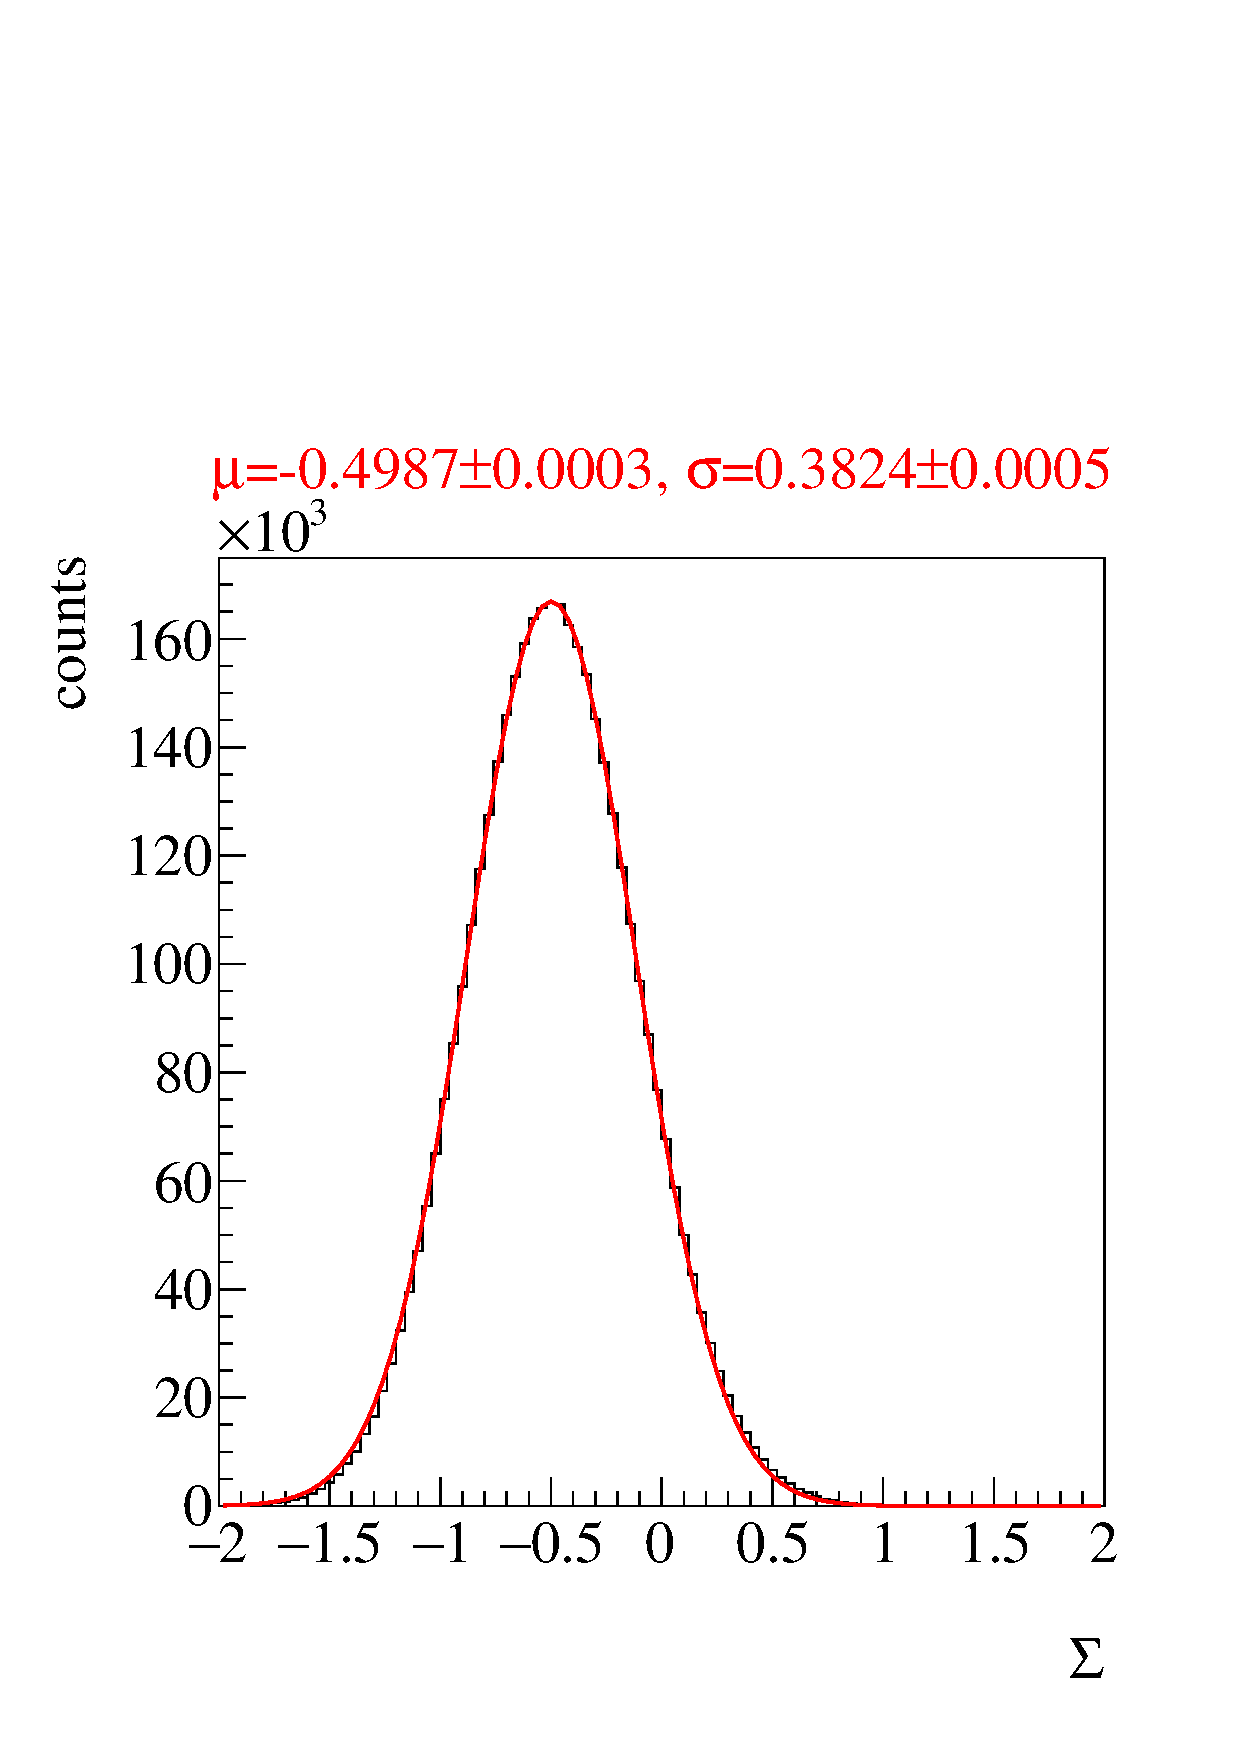
\includegraphics[width=.49\linewidth]{../bayes/etap_event_based_fit/plots/combined_post_add_notrunc_bkg_raw.pdf}
	\subcaption{Background beam asymmetry $\Sigma_t$}
\end{subfigure}
	\caption{Combined posteriors of all 1000 fits without truncation for the signal beam asymmetry $\Sigma_1$ and the background beam asymmetry $\Sigma_t$. Left: normalized residuals $\Xi$, Right: unaltered added posterior distributions. \textsc{Gaussian} fits have been performed with results given on top of each plot.}
	\label{fig:completpost}
\end{figure}
\begin{figure}[htbp]
	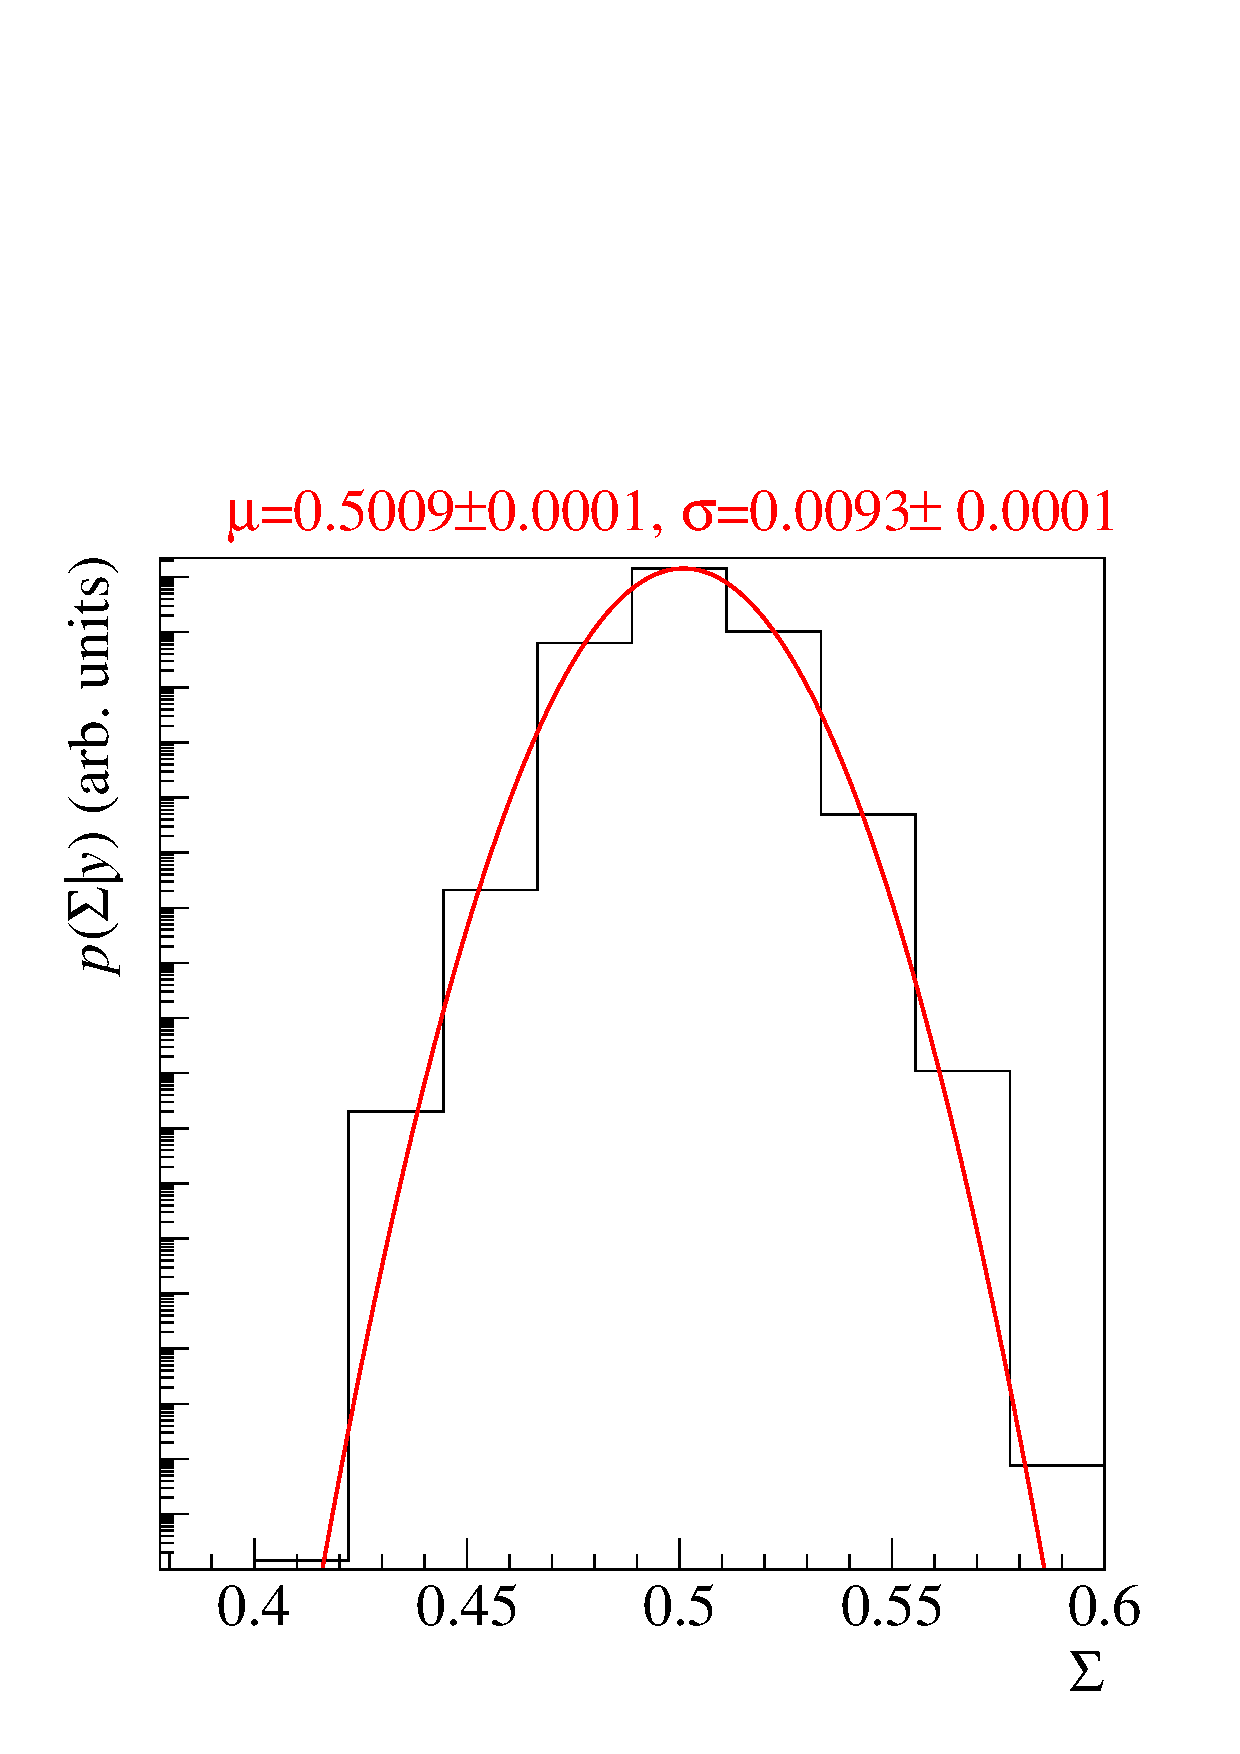
\includegraphics[width=.49\linewidth]{../bayes/etap_event_based_fit/plots/combined_post_mul.pdf}
	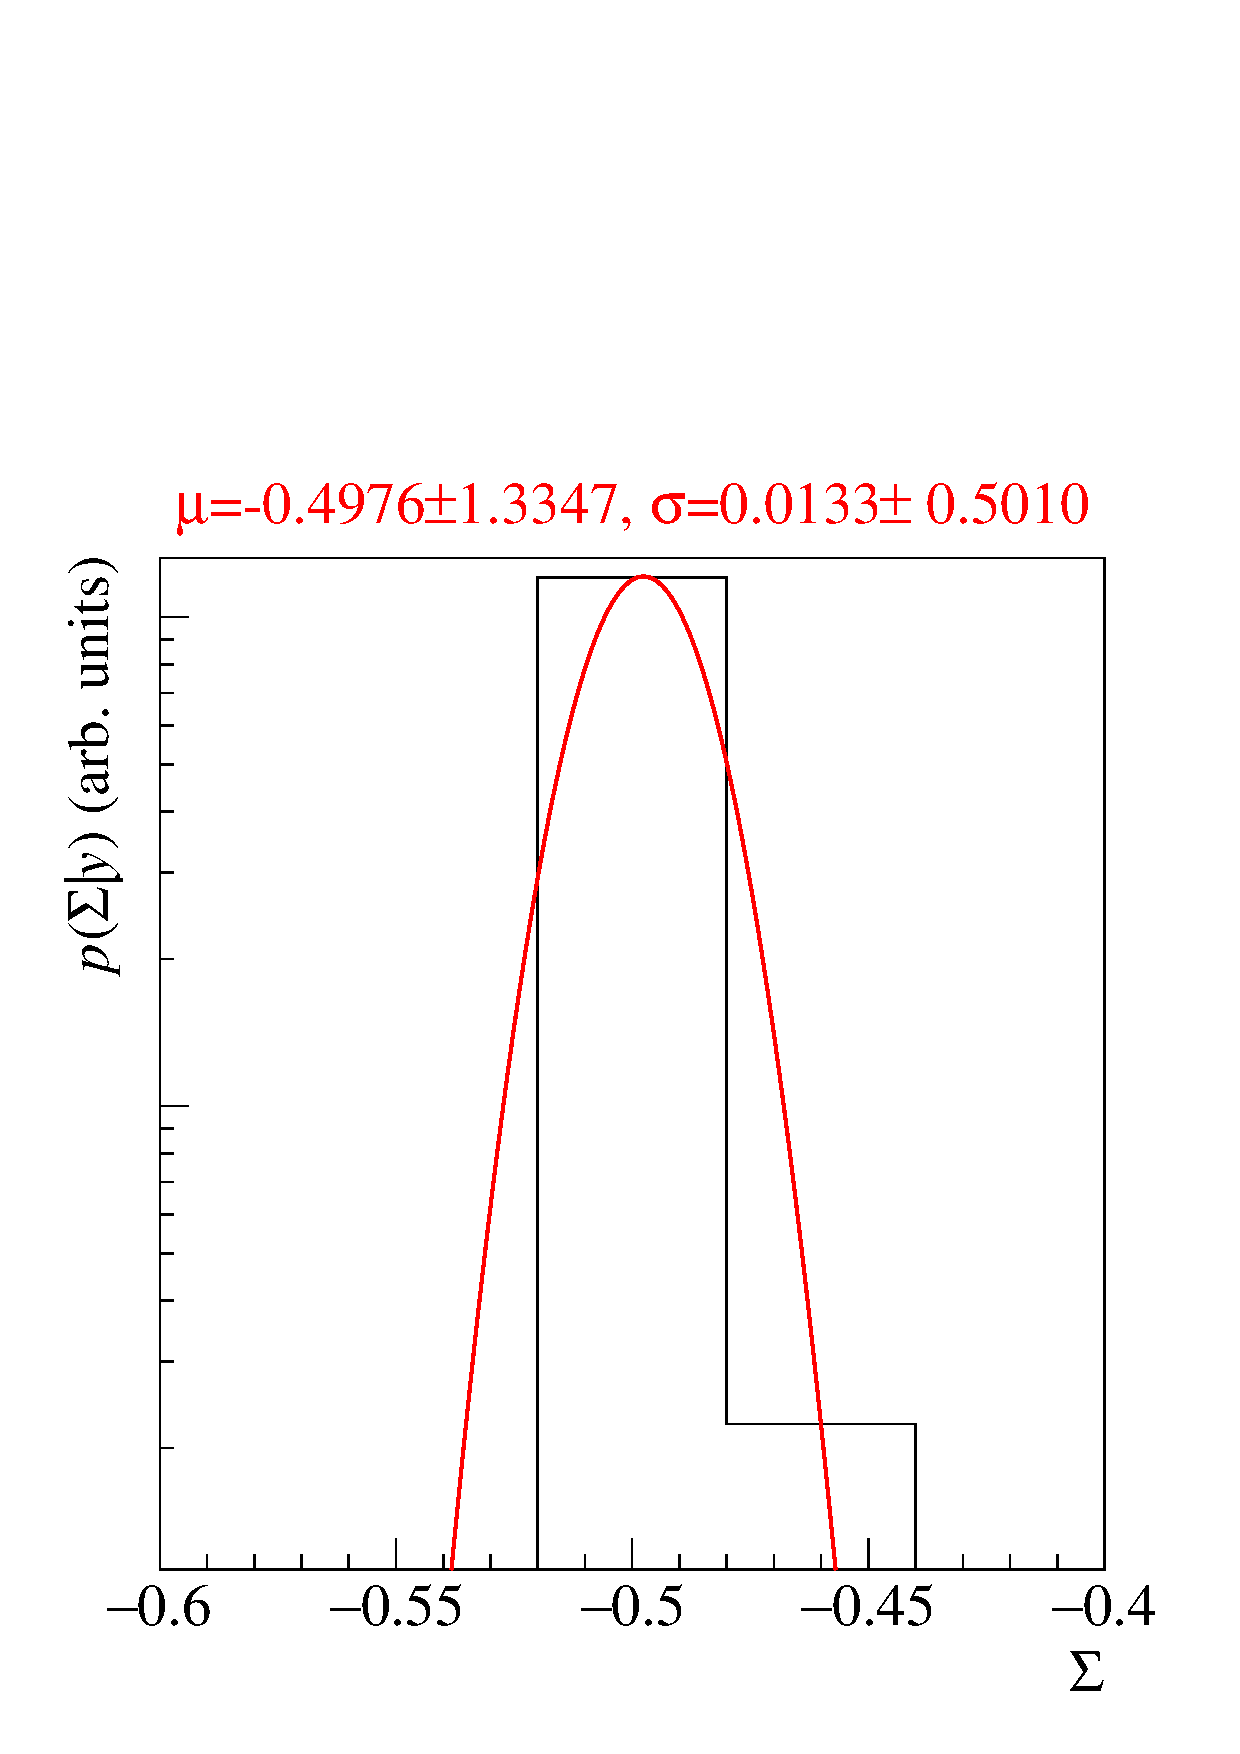
\includegraphics[width=.49\linewidth]{../bayes/etap_event_based_fit/plots/combined_post_mul_bkg.pdf}
	\caption{Posterior distributions of $\Sigma_1$ (left) and $\Sigma_t$ (right) combined in an independent likelihood pool. \textsc{Gaussian} fits to the distribution confirm the reproduction of the input values within $1\sigma$. Note that only very few datapoints were available for the fits, because the distributions overwhelmingly converge into a single bin at $\pm0.5$, hence the large errors on the fit parameters.}
	\label{fig:applik}
\end{figure}





\paragraph{Remark:}
It turned out that without the amount of statistics that was used in section \ref{sec:sigmaeta}, normal priors centered at $0$ for the asymmetries $\Sigma_t$ and $\Sigma$ will mislead the fit results for these parameters towards $0$ if no lower and upper boundaries are used. Instead the priors were then chosen to be uniform on the interval $[-2,2]$. This imposes boundaries, but will not truncate the posteriors because the distributions are not expected to be this wide. All distributions shown here are generated using this model to complete the full investigation of posteriors. Previous toy Monte Carlo experiments (Figure \ref{fig:toyMCpost}) as well as very good agreement between point estimates and posterior distributions (Figure \ref{fig:sigmaetap}) together with the results shown here confirm the validity of the fit used in the main part.
% \printbibliography[heading=subbibliography]

%------------------------------------------------------------------------------
% Use biblatex for the bibliography
% Add bibliography to Table of Contents
% Comment out this command if your references are printed for each chapter.
\printbibliography[heading=bibintoc]

%------------------------------------------------------------------------------
% Declare lists of figures and tables and acknowledgements as backmatter
% Chapter/section numbers are turned off
\backmatter

\listoffigures
\listoftables

%------------------------------------------------------------------------------
% Print the glossary and list of acronyms
% \printglossaries

%------------------------------------------------------------------------------
% You could instead add your acknowledgements here - don't forget to
% also add them to \includeonly above
% %------------------------------------------------------------------------------
\chapter*{Acknowledgements}
\label{sec:ack}
%------------------------------------------------------------------------------

I would like to thank ...

You should probably use \texttt{\textbackslash chapter*} for
acknowledgements at the beginning of a thesis and
\texttt{\textbackslash chapter} for the end.

%%% Local Variables: 
%%% mode: latex
%%% TeX-master: "../mythesis"
%%% End: 


%------------------------------------------------------------------------------
% CV needed when you submit your PhD thesis
% \definecolor{lightgray}{gray}{0.8}
\newcolumntype{L}{>{\raggedleft}p{0.15\textwidth}}
\newcolumntype{R}{p{0.8\textwidth}}
\newcommand\VRule{\color{lightgray}\vrule width 0.5pt}

\thispagestyle{empty}
\section*{Curriculum Vitae}

\subsection*{Personal Details}

\begin{tabular}{L!{\VRule}R}
Name & Johann Schmidt \\
Date of Birth &  \\
Email & abc@physik.uni-def.de \\
Family status & Single
\end{tabular}

\subsection*{Education}

\begin{tabular}{L!{\VRule}R}
1997--2003 & Abitur, ABC Secondary School, Hamburg, Germany\\
2004--2007 & BSc in Physics, Rheinische Friedrich-Wilhelms-Universität, Bonn, Germany.\\
2006 & CERN Summer Student, Geneva, Switzerland. \\
2007--2009 &  MSc in Physics Rheinische Friedrich-Wilhelms-Universität, Bonn, Germany. \\
2009--2012 &  PhD in Physics, Rheinische Friedrich-Wilhelms-Universität, Bonn, Germany. \\
2012 & Advanced Data Analysis School, Frankfurt, Germany.
\end{tabular}

\subsection*{Professional Experience}

\begin{tabular}{L!{\VRule}R}
2004 & Summer Student at CERN, Geneva, Switzerland. \\
2007--2012 & Doctoral work at the University of Bonn, Germany. \\
2008--2009 & Fieldwork at CERN, Geneva, Switzerland.\\
2011 & Talk at the Advanced Physics Conference, Timbucto
\end{tabular}

\subsection*{Languages}
\begin{tabular}{L!{\VRule}R}
German & Mother tongue \\
English & Fluent \\
Russian & Basic
\end{tabular}


\end{document}
